\documentclass[a4paper,12pt]{article}
\usepackage[left=2.54 cm, right=2.54 cm, top=2.54cm]{geometry}

%%% packages from the OUTPUTS
\usepackage[hidelinks]{hyperref}
%\usepackage[utf8,applemac]{inputenc}
\usepackage[round,authoryear]{natbib}

\usepackage{mathtools}

\usepackage{textgreek}
\usepackage[english]{babel}
\usepackage[T1]{fontenc}
\usepackage{lmodern}   %\usepackage[ngerman]{babel}
\usepackage{amsmath, amsthm, amssymb}
\usepackage{fancyhdr}
\usepackage{color}
\usepackage{lastpage}

\usepackage[T1]{fontenc}
\usepackage{array}
\usepackage{multirow}
\usepackage{tikz}
\usetikzlibrary{calc}
\usetikzlibrary{matrix}
\usetikzlibrary{positioning}
\usepackage{titling}
\usepackage{amsfonts}
\usepackage{placeins}
\usepackage{amsfonts}
\usepackage{graphicx}

\usepackage{adjustbox}
\usepackage{float}
\usepackage{dcolumn}
\usepackage{rotating}
\usepackage{lscape}
\usepackage{graphicx}

\usepackage[applemac]{inputenc}
\usepackage[T1]{fontenc}
\usepackage{graphicx}
\usepackage{amsmath}
\usepackage{amsfonts}
\usepackage{amssymb}
\usepackage{array}
\usepackage{pifont}
\usepackage{calc}
\usepackage{xcolor}
\usepackage{hyperref}
\usepackage{caption}
\usepackage{tikz}
\usetikzlibrary{shapes,snakes}
\usepackage{pifont}
\usepackage{amsmath,tabu}
\usepackage[a4paper]{geometry}
\usepackage{ragged2e}
\usepackage{csquotes}
\MakeOuterQuote{"}

\usepackage{longtable}
\usepackage[section]{placeins}

\usepackage{xcolor}
\hypersetup{
    colorlinks,
    linkcolor={blue!50!black},
   citecolor={blue!50!black},
    urlcolor={blue!80!black}
}
%% end of packages from the OUTPUTS

%%%%% from the model

\usepackage[utf8]{luainputenc}
\usepackage{algorithm2e}
\usepackage{amsmath}
\usepackage{amssymb}
\usepackage{setspace}
\usepackage{esint}
\usepackage{booktabs,caption}
\usepackage[flushleft]{threeparttable}

\makeatletter
%%%%%%%%%%%%%%%%%%%%%%%%%%%%%% User specified LaTeX commands.


%%%%%%%%%%%%%%%%%%%%%%%%%%%%%%%%%%%%%%%%%%%%%%%%%%%%%%%%%%%%%%%%%%%%%%%%%%%%%%%%%%%%%%%%%%%%%%%%%%%%%%%%%%%%%%%%%%%%%%%%%%%%%%%%%%%%%%%%%%%%%%%%%%%%%%%%%%%%%%%%%%%%%%%%%%%%%%%%%%%%%%%%%%%%%%%%%%%%%%%%%%%%%%%%%%%%%%%%%%%%%%%%%%%%%%%%%%%%%%%%%%%%%%%%%%%%
\usepackage{amsfonts}\usepackage{subfigure}\usepackage{multirow}

%%% end of packages from the model

%% additional for justification

% --- Title page
\title{Colonial Rule and Economic Freedom
       \bigskip}

\author{Jo\~{a}o Pedro Bastos\thanks{PhD Student, Department of Agricultural and Applied Economics and Free Market Institute, Texas Tech University, Box 45059, Lubbock, TX, 79409-5059. \url{Joao-Pedro.Bastos@ttu.edu}}}

\date{\today}



% ================================================================
% ================================================================
% --- DOCUMENT
\setlength{\marginparwidth}{2cm}
\begin{document}


% ================================================================
% --- TITLE PAGE

\maketitle

\begin{abstract}
\noindent This paper studies the legacy of European colonial rule for economic freedom in former colonies today. Using data on 107 former European colonies, I study how the colonizer's identity and characteristics of the colonial rule -- duration and timing -- are related to economic freedom today. The main results use a historical index of economic freedom to show that the level of economic freedom of colonies is directly related to the level of economic freedom of their colonizers, both at the time of independence and in the twenty-first century. I also find that the length of colonial rule is positively and significantly correlated with average economic freedom from 2000 to 2019. These results are robust to controls for geography, climate, natural resource endowments, the identity of the colonizer, and the timing of colonization.

\end{abstract}

\bigskip \bigskip
\begin{footnotesize}
\noindent \textbf{JEL codes}: N40, O10, P14, P50 \\
\noindent \textbf{Keywords}: colonial rule, economic freedom, institutions, path-dependence
\end{footnotesize}

\clearpage
\doublespacing

% ================================================================
% --- SECTION 1: INTRODUCTION
\section{Introduction} 
    \label{sec:Intro}

Economic freedom is a strong determinant of economic growth and several other measures of development \citep{dehaan2006market,Hall2014,LawsonMiozziTuszynski2024}. Given such relevance for positive outcomes, a large literature has emerged to understand why some countries have more economic freedom than others \citep{lawson2020determinants}. Although it is well-accepted that present-day institutions are developed over long periods of time in a path-dependent process \citep{North1991,spolaore2013deep}, only a few studies have looked closely at the historical dependence of economic freedom. 

In this paper, I study the legacy of European colonial rule for economic freedom in former colonies today. Former European colonies inherited many institutions that were implemented at the time of colonization, notably their legal system, their structure of tax collection, or their land tenure system \citep[e.g.][]{banerjee2005history,Levine2021,laporta1998law,garfias2021fiscal}. Moreover, the characteristics of colonial rule (such as its length, the identity of the colonizer, and the strategy of colonization) presumably affected which institutions were implemented, which in turn shaped current levels of income \citep[e.g.][]{grier1999colonial,Acemoglu2001}. 

Using data on 107 former European colonies, I study how colonial rule characteristics are related to average economic freedom over the period 2000-2019, as measured by the \textit{Economic Freedom of the World} (EFW) Index \citep{EFW_2021}. First, I investigate whether colonizers transmit their levels of economic freedom to their colonies. Using a historical index of economic freedom \citep{prados2016economic} covering the colonial period, I show that countries colonized European nations with greater economic freedom at the time of colonization inherited greater levels of economic freedom today. A colonizer with economic freedom scores one standard deviation higher is associated with a colony that is one-third to one-quarter of a standard deviation freer. This relationship can be seen for all areas of the economic freedom index, except size of government. Being colonized by a freer nation is related to better enforcement of property rights and the rule of law, sound money, more freedom to trade internationally, and less overall regulation.

Second, I find that the length of colonial rule is positively and significantly correlated with modern-day economic freedom. The estimates suggest that every 100 years under colonial rule are associated with roughly a quarter of a standard deviation (0.22 points) higher economic freedom in the twenty-first century. This result is similar in spirit and consistent with those of \cite{grier1999colonial} and \cite{feyrer2009colonialism}, who find that colonies held for longer enjoy higher levels of income today. All sets of results are robust to controls for geography, climate, natural resource endowments, and the identity of the colonizer. Finally, for a smaller sample of countries that gained independence in the second half of the twentieth century, I show that these two main factors -- economic freedom of the colonizer and duration of colonial rule -- explain economic freedom at the time of independence, suggesting that these are not driven by post-colonial reforms.

These results suggest that a country's colonial past is a strong determinant of its modern-day economic freedom and yields tentative implications. First, the difference in modern-day economic freedom associated with being colonized by the freest colonizer (the Netherlands) instead of the least free (Portugal), implies a predicted increase in modern-day per capita income of up to \$10,000.\footnote{Considering the mean effect of the meta-analysis by \cite{lawson2024economic} -- see the discussion at the end of Section \ref{sec:results_efw}.} Further, these results are consistent with the idea that, on the margin, longer colonial tenures support the development of an ``encompassing interest'' from the part of colonizers, which incidentally also rejects a theory of pure exploitation \citep{grier1999colonial} -- or crude versions of both theories, at least. As the time horizon of their dominions is extended, colonizers behave, on average, more like ``stationary bandits'' who invest in better institutions \citep{olson1993dictatorship,Olson2000}. 

This article proceeds as follows. Section 2 reviews the literature on determinants of economic freedom and links it to the literature on the colonial origins of modern-day institutions. Section 3 introduces the data. Section 4 presents the econometric results and the following section discusses their robustness. The last section concludes. 

\section{Literature Review}

Due to its robust association with positive outcomes such as economic growth or human capital, trying to understand why some countries have more economic freedom than others has sparked a large literature reviewed by \cite{lawson2020determinants}. Remarkably, however, only a few studies look far back to historical or geographical facts as a source of today's levels of economic freedom. The first is that of \cite{nattinger2012legal}, which shows that U.S. states that were first settled by civil law countries have less economic freedom today.\footnote{Alabama, Arizona, Arkansas, California, Florida, Louisiana, Mississippi, Missouri, New Mexico, and Texas were first colonized by either France, Mexico, or Spain, and thus originally adopted a civil law legal system.} 

Second, \cite{nikolaev2017historical} test the parasite-stress theory of social values, which posits that the prevalence of infectious diseases shapes the formation of personality traits and cultural values. According to this theory, a higher prevalence of pathogens stimulates collectivist values, which in turn influences the development of economic institutions that undermine economic freedom. They present econometric evidence in support of this hypothesis.

\cite{gohmann2018persistence} develops a variant hypothesis of Diamond's \citeyearpar{diamond1997guns} theory of prevalence of species prone to domestication and East-West orientation of continents, in which these two factors are associated with contemporary levels of economic freedom.\footnote{More precisely, \cite{diamond1997guns} suggests that historical patterns of economic development are determined by three biogeographic factors: (1) existence of crops that allowed self-sufficiency through agriculture, (2) large animals prone to be domesticated that are useful for food, transportation, and agriculture, and (3) a continental landmass oriented mostly in East-West relative to North-South axes, which facilitated migration and transfers of technology across regions with similar temperatures. See \cite{pavlik2019did} for an empirical test of the technology transfer component of the theory.} Gohmann's argument is that societies that adopted agriculture earlier were able to start developing institutions sooner, resulting in more opportunities for the evolution of their institutional frameworks. This, in turn, would lead to the emergence of institutions better tailored to greater economic freedom. While he finds evidence that the two bio-geographical components are related to specific areas of the EFW (see more in Section 3.1), he finds no significant association with the overall economic freedom index.

The last study that analyzes the relationship between geographical determinants and economic freedom is that of \cite{Murphy2021}. He considers many variables suggested by earlier literature, such as a dummy for Eurasia (which captures the East-West element of Diamond), legal origins \citep{nattinger2012legal}, the prevalence of historical pathogens \citep{nikolaev2017historical}, absolute latitude, and  the absolute size of a country.\footnote{The last one is a variant of the work of \cite{alesina2003size}, who argues that countries with large \textit{populations} are more heterogeneous and thus less cohesive, making it harder to devise institutions that promote the common interest or to provide public goods. \cite{Murphy2021} instead focus on \textit{geographical} size, as he argues that population size may be an outcome of geographical characteristics.} The initial findings suggest that "absolute latitude and malaria ecology cause the historical prevalence of pathogens, and pathogen prevalence has a strong effect on economic freedom." He also reports results that show that larger countries (in area) tend to have less economic freedom, and positive relationships between economic freedom and both German and British legal origins. 

Crucially, however, none of these studies addresses the effect of colonial rule, or focus on former colonies exclusively, which, although related, is a question of its own relevance. In contrast, there is a large literature on the colonial origins of historical development that considers the effects of colonial rule on modern-day outcomes, especially income, but not on economic freedom specifically. 

Throughout the Age of Discovery, Europeans conquered territories across the globe, implementing various types of institutions. The Spaniards were famous for their system of \textit{encomiendas}, which granted governing powers over the land and people to the ruling \textit{encomendero}; the French "exported" a centralized rational bureaucracy, sending emissaries and public officials to act as representatives of French government and providers of public services \citep{lockhart1983early,fieldhousecolonial, grier1999colonial}. 

Differences in colonial rule characteristics, in turn, affect present-day outcomes. \linebreak \cite{hall1999some} emphasize how institutions with greater "Western influence" generate higher levels of output per capita in modern times, although their work is not exclusively focused on former colonies. \cite{engermansokoloff1997} develop a similar argument, but condition Western influence on initial factor endowments. For instance, where slave-labor agriculture was feasible, inequality was high because institutions were designed for resource extraction by small colonial elites. \cite{laporta1997legal,laporta1998law,laporta2008economic} argue that the identity of colonizers matters for current outcomes because European powers implemented different legal systems. Their findings show that common-law systems provide greater protection of investors and their property than do systems of French civil-law origins. More recently, though not exclusively focusing on former colonies, \cite{pavlik2021legacy} find that countries whose populations have greater historical experience with representative assemblies have stronger property rights, rule of law, and greater constraints of the executive -- all of which are important elements of economic freedom.

\cite{Acemoglu2001} contend that what determines which institutions will be put in place does not primarily depend on the identity of the colonizer; instead, the institutional environment is mediated by initial settlement conditions for the colonizers. Where they could settle, they developed more inclusive institutions that protected property rights and allowed investments in human and physical capital, which in turn determined today's income levels. \cite{bennett2017economic} diverge from \cite{Acemoglu2001} by contending that colonizer identity and settlement conditions should be treated as complements rather than substitutes. They also posit that geography exerts both direct and indirect effects on post-colonial development paths. 

Closer to this study is that of \cite{grier1999colonial}, which was the first to consider the relationship between the length of colonial rule and modern outcomes. Similarly to the present study, her results show that colonies held for longer present higher economic growth and have higher levels of income. Although \cite{grier1999colonial} recognizes that this is not a causal effect, it helps in rejecting a "crude form of exploitation theory." This hypothesis was revisited by \cite{feyrer2009colonialism} for a sample of islands, finding similar evidence. Because the length of colonization could be a consequence of selection whereby ``colonizers may settle the best places first and give them up last,'' the authors instrument years under colonial rule with the speed and directions of winds, which exogenously determine which islands were first found by European navigators. Their results strengthen the idea that the length of colonial rule is associated with modern income levels.

The present study connects these two strands of the literature by analyzing the relationship between colonial rule and economic freedom today. In this regard, I expand the work of \cite{laporta1997legal,laporta1998law,laporta2008economic}, and \cite{engermansokoloff1997}, by showing that even after controlling for the identity of colonizer and initial geographical characteristics, the length of colonial rule is still a strong determinant of modern outcomes. I also complement the work of \cite{grier1999colonial} and \cite{feyrer2009colonialism} by including an institutional link -- namely, economic freedom -- between colonial tenure and modern-day levels of income.

\section{Data}

\subsection{Economic Freedom of the World Index}
\label{sec:efwdata}

Estimates of economic freedom come from two sources. Modern-day economic freedom for colonies comes from the Economic Freedom of the World (EFW) Index \citep{EFW_2021}. Conceptually, the EFW  measures the degree to which economic activity is guided by voluntary transactions in the market, free from government constraints.\footnote{``Central planning and allocation of resources by political processes, are government activities that reduce the overall level of economic freedom. However, the government plays an important role in protecting property rights and providing access to fair courts to resolve disputes.'' \citep[p. 1]{EFW_2021}.} It is comprised of five areas that receive equal weight: Size of Government, Legal System and Property Rights, Sound Money, Freedom to Trade Internationally, and Regulation. Data ranges from a minimum of 0 to 10 (most free) and is available in five-year intervals from 1970-1995, and annually since 2000. \cite{murphy2018extending} also provide an extension of the data back until 1950, but with a smaller number of variables under each area.

I use the EFW to construct four outcome variables for the colonies. The main variable of interest is the average economic freedom for the 2000-2019 period ($Avg.$ $EFW$). There is considerable variability in the index, ranging from a minimum of 3.92 (Sudan) to 8.38 (Singapore); the mean is 6.13 and represents a country like Swaziland or Zambia. 

Second, for a reduced number of countries ($n$ = 54) that gained independence since 1941, I am able to obtain their economic freedom score at (or close to) the time of independence. I consider these countries eligible if they obtain a score within 10 years of independence. The late independence sample contains observations from all continents, but not all colonizers, as no former Portuguese, Spanish or Italian colonies fit the criteria.\footnote{Relative to the base sample, it includes more observations from Africa (59.3 vs. 44.9\%) and less from America (26.17 vs. 11.1\%). Oceania and Asia shares are roughly the same in both samples. French colonies are proportionally more prevalent in the late independence group (35.2 vs. 25\%) and all four German colonies are present in both groups. See Table \ref{tab:TableA1} for summary statistics by colonizer and by continent.}

Third, I construct the $\Delta EFW$ variable, which measures the change from a country's first EFW\footnote{For countries that gained independence since 1941, this will be their EFW at the time of independence. For countries that became independent earlier, this will be the first year for which a score is available.} to its score in 2019. Although most countries (88\%) increased their scores over time, I use this measure as a robustness check, as discussed in Section \ref{delta}.

Finally, I create a variable called $EFWStd$. I use this to test whether countries that had more than one colonizer have a less "cohesive" EFW score, presumably because multiple colonizers across time can implement different institutions that are not functionally connected. This follows the spirit of \cite{bolen2020does}, who find that countries with a smaller standard deviation (i.e. more cohesiveness) among the areas of EFW have larger rates of growth. Summary statistics for all variables are available in Table \ref{tab:Tab1}.

\subsection{Historical Index of Economic Liberty}\label{sec:HIEL}

Historical data for the European colonizers comes from The Historical Index of Economic Liberty (HIEL) \citep{prados2016economic}. It provides economic freedom scores for OECD countries starting in 1850 until the present day. Although it omits the "Size of Government" area, the four remaining areas of the index are inspired by and otherwise follows the same structure of the EFW described above. Of the 15 variables in the four sub-indices, seven come from the V-Dem project \citep{coppedge2019methodology}, and the remaining are proxied by national accounts series from economic history literature.\footnote{V-Dem variables are concentrated mostly in the sub-areas of Legal System and Property Rights, and Regulation. Data for sound money and international openness are from historical national accounts. For instance, data on tariffs is implied by the ratio of total tariff revenue over total export and import value.} 

For each colony, I calculate the economic freedom of their colonizer as the average HIEL score over the period of colonization with available data. For instance, for a British colony between 1800 and 1900, the economic freedom of the colonizer will be England's average HIEL score from 1850 (first year with available data), until 1900.\footnote{To check for potential biases arising from the pre-1850 omitted period, I also include a specification focusing only on those countries colonized after 1850. Results are largely unchanged.} Countries that gained independence before 1850 are excluded from this sample, as no information about the economic freedom of their colonizer can be obtained. Using this method, the Netherlands had the highest HIEL score (7.96) during its time as a colonizer, followed closely by Britain with 7.81. The remaining are Belgium (7.47), Germany (7.42), France (7.06), Spain (6.52), Italy (6.36), and Portugal (6.34).

\subsection{Historical and Geographical Data}
\label{sec:HistoricalData}

Historical data for this paper comes from multiple sources. The main one is the Colonial Dates Dataset \citep{COLDAT}, which is used to identify former European colonies and construct variables such as the duration of colonial rule. It includes 128 former colonies of Belgium, Britain, France, Germany, Italy, Netherlands, Portugal, and Spain. However, 21 colonies for which there is EFW data is not available were dropped.\footnote{The majority of which being small islands of the Pacific or Indian Oceans, but also Cuba, Dominica, Eritrea, and Equatorial Guinea.}

On average, these countries remained 170 years under colonial rule, but the range is quite large, ranging from 15 (Iraq) to 513 years (Cabo Verde). An advantage of using this dataset is that it allows for more precise estimates of the length of colonial rule under \textit{each} European nation. For instance, \cite{grier1999colonial} uses the date of independence minus the date of arrival of the first European nation. However, several colonies had temporary independence at some point in the interim -- averaging 52 years -- between two colonial rulers. Further, while most countries were colonized by a single European nation, roughly twenty percent of the colonies had two colonizers, and two of them had three. 

For the 23 cases with multiple colonizers, identifying the ``main'' one merits some discussion. Is the main colonizer the one that ruled for longer? Or are there other criteria for defining the most important one? In general, I follow the same classification as \cite{laporta1999quality},\footnote{This is also the classification used in \cite{Acemoglu2001,acemoglu2002reversal}.} except for Seychelles, which does not appear in their sample and I code it as a former British colony. In 7 of the 23 cases, the main colonizer is also the longest. For instance, this is the case of Uruguay, which remained 142 years under Portuguese domain, but 233 years under Spain. The classification is sensible in this case: the Portuguese hardly settled the territory, Uruguay eventually gained independence from Spain and is a Spanish-speaking country today. 

However, in cases such as Canada, South Africa, and Malaysia, which respectively have been colonized for the longest by France, the Netherlands, and Portugal, it would be inaccurate to classify these as the \textit{main} colonizers. The French and Dutch controlled only a minority of the Canadian and South African territories; Malaysia was a trade outpost for the Portuguese between 1511 and 1641, but arguably this is much less influential than the British domain between 1847 and 1958, although the latter is shorter (111 vs. 130 years). Table \ref{tab:Tab2} provides the main classification used for each country. Importantly, as shown in Appendix Table \ref{tab:TabB4}, the main results hold if colonizer identity is coded as the \textit{longest} colonizer.\footnote{Table \ref{tab:classification} compares the classification of colonizer identity using the longest-ruler criterion and the one used for the base sample.}

I also use data on geographical and pre-colonial characteristics to control for selection bias in colonial tenure, whereby colonizers may settle the colonies with the largest potential first and give them up last. The set of geographical characteristics includes five indicators of temperature, four indicators of humidity, six indicators of climate/soil quality, and five indicators for the presence of natural resources (gold, iron, silver, zinc, and oil reserves), all from \cite{parker1997national}. I also include two dummies for whether a country is landlocked and whether is an island \citep{dkpublishing1997world}, to account for better access to maritime trade routes, and data for pre-colonial population density from \cite{mcevedy1978atlas}.\footnote{All of which as available in \cite{acemoglu2002reversal}.}

%The basic argument is that European colonialism resulted in the establishment of private property institutions in regions that were previously economically disadvantaged (and thus less densely populated), while simultaneously introducing or perpetuating extractive institutions through indirect colonial rule in areas that had been prosperous, but that Europeans could not settle due to the disease environment. 
\section{Results}

\subsection{Economic Freedom of Colonizer}\label{sec:results_efw}

The main results speak to the relationship between the economic freedom of the colonizer and the colonized and are reported in Table \ref{tab:Tab3}. The dependent variable is the average EFW score of the former colony for the 2000-2019 period, and the main explanatory variable is the average HIEL score of their colonizer over the period in which it colonized that country. Since HIEL data is available only from 1850 onwards, this sample omits countries that gained independence before 1850.

Column 1 relies on a "naive" regression with no controls, while subsequent columns address potential issues. The results show that the freer the colonizer during the colonial era, the freer the colony is today. Since the measure of average HIEL scores is based on years from 1850 onwards, column (2) excludes countries before that year to assure that averages represent the totality of the colonization period and do not omit any years. Results are largely unchanged. Columns (3)-(6) consider whether the results may be driven by specific regions. Excluding Africa (3) reduces the sample by more than half (to 39 observations), and results become statistically insignificant.\footnote{Below, in section \ref{sensitivity}, I show that this is not caused by Africa driving the results, given that all colonies receive similar regression weights. Likewise, column (5) show that including continent dummies does not affect the significance of the results.}  Estimations without the Americas (4) and "Neo-Europes" (Australia, Canada, and New Zealand).\footnote{The United States is not in this sample because it became independent before 1850.} 

Column (7) controls for location, including absolute latitude and two dummies for land-locked and island colonies. This aims to control for environmental factors (e.g. climate, disease environment) that may condition settlement patterns \citep[e.g.][]{Acemoglu2001,Sachs2003,engermansokoloff1997}. Column (8) controls for the timing of colonization. \cite{feyrer2009colonialism} argue that countries colonized after the Enlightenment counted with much more benevolence on the part of the colonizers, especially towards native populations. The results presented here, however, suggest that the opposite, at least in terms of institutions related to economic freedom. Colonies where Europeans arrived later have, on average, lower EFW scores in the modern era. Being colonized 100 years later is related to a 0.2 lower average EFW score. Nevertheless, all results point out to a strong positive relationship between the economic freedoms of colonizer and colonized. The point estimates suggest that colonies "inherit" 45 to 71 percent of their colonizer's economic freedom score. 

To put the economic significance of these results in perspective, consider the following example. If, instead of being colonized by Portugal, Brazil had been colonized by the Netherlands -- an implied increase of 1.59 points in the average economic freedom of the colonizer -- we would expect Brazil's modern-day average economic freedom to be 1.16 points (1.21 st. dev.) higher. This would place Brazil in the top 50 most free countries, instead of more than 60 positions below, ranking at 113. More importantly, if we consider the average effect of economic freedom on income reported in the meta-analysis by \cite{lawson2024economic}, this increase in economic freedom implies that Brazil's per capita income would be around \$8,500 to \$10,600 higher, which would be sufficient to double its current per capita income (around \$8,900).\footnote{\cite{lawson2024economic} report that a one standard deviation increase in EFW (around 0.96 points) is related to a 0.4 to 0.5 standard deviation increase in income (around \$17,500).}

\subsection{Length of Colonial Rule}

The next set of results tests the relationship between colonial tenure and modern-day economic freedom and is presented in Table \ref{tab:Tab4}. Column 1 starts with a simple regression of $Avg. EFW$ on the number of centuries that a country remained as a colony. The estimate suggests that each additional century (or 0.9 of a standard deviation) of colonial rule is associated with a 0.221 higher average EFW score, or nearly a quarter of a standard deviation. 

One potential explanation for this positive relationship is that it may reflect a simple underlying correlation between the identity and tenure of the colonizer: colonizers that tended to hold their colonies for longer also tended to have more liberal economic institutions or a better legal system. In column (2) and in subsequent columns, I include a dummy for each colonizer to restrict the analysis to within-colonizer variation and to account for other time-invariant and colonizer-specific unobservables. The inclusion of colonizer fixed effects does not change the results, although they are less precisely estimated.\footnote{The values for the colonizer dummies are available in Table \ref{tab:TabB2}, Column (7). Belgium is the baseline.}

Removing Africa in column (3) reduces the sample size by 45\%, and the coefficient on centuries of rule ceases to be significant. Leaving America out in column (4) yields a point estimate similar to (2), but it is only significant at the 10\% level. The more imprecisely estimated coefficients are likely due to the small sample size. This is in part reassured by the fact that, in column (5), the inclusion of continent dummies retains significance. Also, given that "Neo-Europes" are strong outliers,\footnote{Excludes Australia, Canada, New Zealand, and the United States which (together with Singapore) are all among the top EFW scores in the base sample.} and to ease concerns that these observations may be driving the results, I exclude them from the estimation in Column (6). Nevertheless, the results remain significant. 

Still, there are many other possible concerns with the initial results. The main one is selection by the colonizers. The "discovery" of colonies was not entirely random. Some colonies situated along the main historical trade routes were already known to Europeans (e.g. Middle East and North Africa). But accident also played a large role, as Columbus reached the Lesser Antilles in 1493 and Amerigo Vespucci declared it the New World. At least in the case of islands, \cite{feyrer2009colonialism} argue their discovery were largely influenced by exogenous factors such as the speed and direction of winds in navigation. 

However, "discovery" and actual colonization are not clearly connected. For instance, North Africa was of course already known for millennia prior to the Age of Discovery, but it was colonized in the mid to late nineteenth century. Even if we assume that colonies were randomly \textit{found}, selection would still be present as Europeans chose to colonize the most important first, and \textit{keep} the best colonies for longer. Those along coastal Africa were quickly recognized as important maritime trade posts. Thus, it is not by accident that the Cabo Verde was colonized in 1462 and Ghana in 1476 -- the first two in the sample. More broadly, it is likely that colonizers kept colonies with better potential for land productivity, natural resources, weather, or strategic geography to serve as trade outposts. 

With that in mind, I use a series of controls to explore the robustness of my results.\footnote{As a robustness check, I consider this hypothesis more carefully in Section \ref{selection}.} Column (7) starts by controlling for the location characteristics of the colonies. While the dummy for whether the colony is land-locked is not significant, both latitude and island status are positively related to present-day levels of economic freedom. Given their moderate temperatures and reduced prevalence of tropical diseases, greater absolute latitudes provided more amenable settlement conditions for Europeans, as argued in different flavors in (e.g.) \cite{hall1999some}, \cite{Acemoglu2001}, and \cite{bennett2017economic}, so the sign behaves as expected. The island dummy provides support for \cite{fors2014island}, who argued that island status improves institutional quality by increasing social cohesion. Crucially, the length of colonial rule remains significant and positive, albeit smaller in magnitude, when these controls are included. 

Column (8) includes several controls for temperature, humidity, and weather/soil (e.g. desert, steppe, highland) that aim to capture differences in land productivity. Including these controls does not substantially alter the results.\footnote{I report the \textit{p}-values for the null hypothesis that each group of indicators is not significant. Only climate/soil is significant, though it could be due to its strong correlation (by construction) with varying levels of absolute latitude.} Finally, column (9) includes controls for the presence of natural resources, namely gold, iron, silver, and oil reserves; these are joint-significant at the 1\% level, but leave the coefficient of interest largely unchanged.  


\subsection{Timing: Evidence from Late Independence}\label{sec:late}

Since the main dependent variable averages economic freedom for the 2000-2019 period, a question that arises is to what extent these results arise directly (or immediately) from the colonial era. In other words, were the colonizers themselves that implemented institutions compatible with economic freedom? Alternatively, is there some underlying factor that is related to colonial rule tenure and also determines reforms in the post-colonial period (i.e. following independence) that eventually lead to greater economic freedom in the modern era? 

This section wishes to adjudicate these hypotheses by looking at countries that gained independence later, from the 1940s onwards. The intuition is simple. If we are able to identify correlations between colonial rule characteristics and economic freedom immediately following independence, it is unlikely that greater economic freedom was mainly achieved through economic reforms following independence. 

For this exercise, I produce estimates analogous to the results of Tables \ref{tab:Tab3} and \ref{tab:Tab4}, but with one difference: instead of the average EFW score in the 21st century, the dependent variable becomes the very first EFW score following independence. I use the extension of the EFW developed by \cite{murphy2018extending}, which provides data back until 1950, though relying on a small number of variables in each area of the EFW. This reduces the sample to those countries that obtained an EFW score within 10 years of independence and thus gained independence in 1940 or later (see Section \ref{sec:efwdata} for details). 

Table \ref{tab:Tab5} reproduces the results linking economic freedom scores of colonizers and colonized. Interestingly, significant point estimates are even larger than the ones considering average economic freedom in recent times. For each additional point in economic freedom scores of the colonizer, colonies "inherit" 0.777 to 1.106 points in their EFW score following independence. The estimates are mostly significant, except for columns (2) and (3). As in the main sample, when African colonies are excluded, the relationship becomes insignificant, likely due to a very small number of only 22 observations. The lack of significance in column (3) is likewise caused by a small $N$. Including a dummy for colonization post-1850 (instead of dropping the observations) retains the significance of the main explanatory variable. Likewise, including continent dummies instead of dropping Africa retains significance in column (5).

In Table \ref{tab:Tab6}, I report the results considering the length of colonial rule. Column (1) starts with the simplest specification, without any controls. The positive relationship is significant and in fact stronger than for the full sample. Column (2) repeats the exercise while controlling for the identity of the colonizer, which yields results in line in magnitude with the base sample, and significant at the 10\% level. I follow by adding similar sets of controls as for the base sample. I remove African colonies in column (4) and American colonies in (5). Only the former retains significance. Including continent dummies in column (5), as well as timing (6), location (7), and climate (8), all lead to insignificant results. 

These results, of course, should be interpreted with caution, for two reasons. First, it is not clear whether they can be generalized to colonies that gained independence earlier. Second, while it suggests that differences economic freedom are related to the duration of colonial rule from the time of independence, results are not as robust to additional sets of controls as in the main sample. However, it should also be noted that most specifications are very demanding given the number of observations and thus less likely that any potential relationship retains significance.\footnote{For instance, removing colonizer fixed effects makes the coefficient of interest in columns (6) and (7) significant, while that of column (8) is just outside of the usual significance threshold (\textit{p} = 0.108).} In section \ref{delta}, I provide further robustness checks related to these results.

\subsection{Individual Areas of EFW}

While I find evidence for an overall relationship between how free was the colonizer and how free became the colony, it is unclear whether this relationship holds for all areas of the EFW index. In Table \ref{tab:TabB1}, I answer this question by regressing the average score (2000-2019) of each of the five areas of the colonies' EFW score on their colonizer's HIEL score (at the time of colonization). Table \ref{tab:TabB1} shows that colonies ruled by freer colonizers score better on each of the individual areas of the EFW index, although the results for Size of Government (1) are not statistically significant.\footnote{This results make sense, since HIEL omits the Size of Government area.} However, I find no evidence that freer colonizers are related to a smaller standard deviation among the individual areas.

Table \ref{tab:TabB2} reproduces an analogous exercise for the individual areas of the EFW, but using the duration of colonial rule as the main explanatory variable. Using the baseline specification of Table \ref{tab:Tab4}, column (2) (i.e. controlling for colonizer fixed effects), I find that countries colonized for longer have smaller governments (1), better enforcement of property rights and a stronger rule of law (2), and less overall regulation of their economies (5). Results for sound money and freedom of international trade are also positive, but not significant. Finally, column (6) also shows that colonies held for longer also have lower standard deviation between the five areas of EFW. This result is consistent with the idea that longer colonial tenure allowed the colonizers to implement more cohesive institutions. 


\section{Robustness Checks}

Apart from the numerous specifications presented along the main results, this section provides some additional robustness checks that strengthen the confidence in the previous results. 


\subsection{Sensitivity Analysis}\label{sensitivity}

In Figure \ref{fig:FigB1}, I plot the relative weights from the regressions in Column (1) of Table \ref{tab:Tab3} and Column (2) of Table \ref{tab:Tab4}, in the spirit of \cite{aronow2016does}. It shows that the main results are not driven by any colony in particular, with a smooth distribution of implicit weights across all observations. More precisely, no observation provides more than 1.73\% of the implicit weights for the coefficient of interest in either specification. This also dissuades concerns that the lack of significance in specifications without Africa may be caused by colonies in that continent driving the overall results.

\subsection{Selection}\label{selection}

As discussed earlier, it is intuitive that colonizers would decide to settle the best colonies first and give them up last. Colonies along maritime trade routes, with fertile soil and amenable climates, or with plenty of natural resources are likely candidates for extensive colonization. Along with the numerous specifications that attempt to control for these potential selection effects in the previous section, here I provide some additional evidence.\footnote{In the Supplemental Materials, Table \ref{tab:TabB7}, I also discuss the determinants of colonial tenure.} 

First, I control for pre-colonial population density, calculated by dividing total population by total arable land, thus mainly excluding inland water, desert, and tundra. This is an important control because ``only areas with high agricultural productivity and a developed transportation network can support large urban populations.'' \citep[][p.1232]{acemoglu2002reversal}. Thus, large population densities are indicative of areas more susceptible to settlement and with greater labor force, both of which could be desirable by colonizers.\footnote{Indeed, I show below in Table \ref{tab:TabB7} that this variable is a strong determinant of timing and length of colonization.} Table \ref{tab:TabB3} reproduces the main results (Tables \ref{tab:Tab3}-\ref{tab:Tab6}) with the inclusion of this variable. They are mostly unchanged in terms of magnitude and significance for columns (1) and (3), where the main explanatory variable is the economic freedom of the colonizer. In columns (2) and (4), where I consider the length of colonial rule, the results are stronger -- larger point estimates and greater significance.

Finally, in columns (5) and (6), I test whether any additive and multiplicative relationships exist between the economic freedom of the colonizer and the length of colonial rule. The first implicitly controls for selection to the extent that if colonizers kept the ``best'' colonies for longer, then any economic freedom results could be biased because they capture the colonies in which colonizers invested more time to devise better economic institutions. It also controls for any potential correlation between the economic freedom of colonizer and the average length of their colonial tenures. In any case, the results suggest that these relationships persist independently of each other over the relevant change of these variables. 

Column (6) test whether these variables have multiplicative effects. That is, do economically free colonizers make their colonies ever freer if they stick with them for longer? This hypothesis is rejected by the lack of statistical insignificance on the interaction term. The fact that the coefficient of centuries of rule ceases to be significant suggests that in the extreme case where the economic freedom score of the colonizer is zero, additional years under colonial rule are unrelated to average economic freedom. 

\subsection{Longest Colonizer}

In Table \ref{tab:TabB4}, I show that the results for the length of colonial rule do not change if countries with multiple colonizers are assigned to their \textit{longest} colonizer instead of their main colonizer.\footnote{See the discussion in section \ref{sec:HistoricalData} and Table A2 for the alternative classification of countries according to their longest colonizers.} In all columns the results remain statistically significant and of similar magnitudes as those of Table \ref{tab:Tab4}.

\subsection{Changes in Economic Freedom over Time}\label{delta}

In section \ref{sec:late}, I show that the relationship between both the economic freedom of the colonizer and the tenure of colonial rule to the economic freedom of the colonies can be seen immediately following independence. This suggests that greater economic freedom is not majorly determined by reforms in the post-independence period. To increase the confidence in those results, Table \ref{tab:TabB5} shows that neither freer colonizers nor the duration of colonial rule are related to \textit{changes} in economic freedom after independence. Indeed, most of the variation in economic freedom explained by colonizer and colonial rule characteristics is present as early as the time of independence, instead of driven by post-colonial reforms.

\subsection{Multiple Colonizers and Institutional Cohesion}

Finally, I test how being colonized by more than one nation (either simultaneously or across time) affects current levels of economic freedom. \cite{bolen2020does} show that the standard deviation among the areas of EFW is a strong predictor of growth. Because several colonizers can potentially focus on implementing different institutions across time, countries under multiple colonial rulers could develop dysfunctional or incoherent institutional environments. Table \ref{tab:TabB6} regresses the 2000-2019 average of within-year standard deviations across the five areas of the EFW, on an indicator for countries with multiple colonizers. I also include colonizer fixed effects and control for the centuries of rule in columns (2) and (3). Results can be interpreted as showing no evidence for this hypothesis. If anything, it would suggest the opposite, as all three specifications sign is negative, but significant only in column (2).

\section{Conclusion}

Institutions consistent with greater economic freedom are important predictors of economic growth and development. As such, research on the determinants of economic freedom has been receiving the attention of several scholars \citep{lawson2020determinants}. However, institutions usually develop across long periods of time \citep{spolaore2013deep}, and are often constrained by historical accidents in a path-dependent process \citep{North1991,page2006path}. This paper connects these two literatures by studying the relationship between modern-day economic freedom and characteristics of colonial rule among former European colonies. 

These findings suggest two main takeaways. First, colonies that were colonized by European nations with greater historical economic freedom are freer today. This relationship is sizeable and robust to numerous controls for geographical characteristics, such as climate, soil fertility, and presence of natural resources.\footnote{Incidentally, I also find strong support for \cite{fors2014island}, who argues that greater social cohesion in islands leads to better institutional quality. Indeed, in all specifications where a dummy for islands was included, it correlated strongly with greater economic freedom.} This relationship is also positive and significant for each of the individual areas of the EFW index, except Size of Government.  

Second, longer colonial rule is also related to greater economic freedom today. This finding is particularly relevant because it helps to provide an institutional mechanism for why colonies held for longer have larger incomes today, as in \cite{grier1999colonial,feyrer2009colonialism}. Colonies held for longer have more economic freedom, and more economic freedom leads to greater income levels \citep{dehaan2006market,lawson2024economic}. 

Two contentions are in order. While this paper highlights that the relationship between the levels of economic freedom of colonies and their colonizers can be observed immediately following independence, the transmission mechanism is still unclear. Additionally, why longer colonial tenures lead to better institutions (or income) is still an open question. However, they are consistent with a crude version of the ``stationary bandit'' hypothesis \cite{olson1993dictatorship}, whereby a longer time horizon incentivizes the development of an encompassing interest. Also, as highlighted in similar research by \cite{grier1999colonial}, it rejects a crude version of pure exploitation on the part of colonizers. Further explorations of these questions could be addressed in future research. 

% ================================================================
%    REFERENCES
\clearpage
\singlespacing
\bibliographystyle{apalike}
\bibliography{ref}
%\setlength\bibitemsep{1\itemsep}

% ================================================================
%    TABLES AND FIGURES -- RESULTS
\clearpage
\centering
\section*{Tables and Figures}

\setcounter{table}{0}
\setcounter{figure}{0}

\begin{table}[h!]
\centering
\begin{threeparttable}
\caption{Summary statistics}\label{tab:Tab1}
\begin{tabular*}{\textwidth}{@{\extracolsep{\fill}}lccccc@{\extracolsep{\fill}}}
\midrule
\midrule
\multicolumn{6}{c}{Base Sample}\\
\midrule
 Var. & Obs       & Mean   & Std. dev. &      Min    &    Max \\
\midrule
HIEL Colonizer & 87 &   7.463   & 0.514   & 6.342  & 8.416 \\
Years of rule & 107 & 162.6 & 120.858 & 15 & 513 \\
Year of Independ. & 107 & 1930.6 & 56.783 & 1781 & 1984 \\
$Avg.$ $EFW$ & 107 & 6.442 & 0.959 &  3.860  & 8.751 \\
$EFWStd$ & 104 & 0.264  &  0.171 &  0.068 &  1.031 \\
$\Delta EFW$ & 107 & 1.115 & 1.056 & -3.432 & 3.562 \\
EFW (2019) & 107 & 6.587 & 1.003 & 2.871 & 8.810 \\
\midrule
\midrule
\multicolumn{6}{c}{Late Independence} \\
\midrule
Var. & Obs & Mean & Std. dev. & Min & Max \\
\midrule
HIEL Colonizer &  54  &  7.498  &  0.408 &  6.369 &   7.987\\
Years of rule & 54 & 132.4 & 111.575 & 22 & 456 \\
Year of Independ. & 54 & 1960.1 & 8.106 & 1941 & 1980 \\
$EFW$ $Indep.$ & 54 & 5.178 & 1.001 &  3.621  & 7.613 \\
$EFWStd$ & 54 & 0.750 & 0.324 & 0.175 & 1.567 \\
$\Delta EFW$ & 54 & 1.354 & 0.932 & -0.776 & 3.457 \\
EFW (2019) & 54 & 6.532 & 0.900 & 4.719 & 8.810 \\
\hline
\hline
\end{tabular*}
\begin{tablenotes}
\small
\item \textit{Notes}: HIEL Colonizer is the average \textit{Historical Index of Economic Liberty} score of the colonizer during the time of indepedence. Countries that gained independence before 1850 are excluded from the sample. The \textit{Economic Freedom of the World} (EFW) Index scores ranges from 0 to 10. $Avg.$ $EFW$ is the average score in the 2000-2019 period. $EFWStd$ is the standard deviation between the individual scores for the five areas of the index. $\Delta EFW$ is the difference between either the first available EFW score or the score at the time of independence (for countries that gained independence after 1940) and the 2019 score. The late independence sample contains only former colonies that gained independence since 1940 and obtained an EFW score within 10 years of independence. $EFW$ $Indep.$ is the first EFW score within 10 years of independence.
\end{tablenotes}
\end{threeparttable}
\end{table} % Sum Stats

\clearpage
\begin{table}[h!]
\centering
\begin{threeparttable}
\caption{List of Former Colonies with Available EFW Data, Base Sample}\label{tab:Tab2}
\begin{tabular*}{\textwidth}{@{\extracolsep{\fill}}lll@{\extracolsep{\fill}}}
\hline
\hline
            \textbf{Belgium: 1}     &              \textbf{Britain (cont.)} &               \textbf{France (cont.)} \\
            Dem. Rep. of the Congo	&	                       Singapore 	&	                         Tunisia 	\\
            \textbf{Britain: 49}	&	                         Somalia* 	&	                            Vietnam	\\
                        Australia 	&	                       South Africa	&	                \textbf{Germany: 4}	\\
                         Bahamas 	&	                       Sri Lanka 	&                         	Burundi*	\\
                         Bahrain 	&	                           Sudan 	&	                        Cameroon*	\\
                      Bangladesh 	&	                       Swaziland 	&	                            Rwanda*	\\
                        Barbados 	&	                        Tanzania 	&	                        Tanzania*	\\
                          Belize 	&	               Trinidad \& Tobago* 	&                 	\textbf{Italy: 1}	\\
                          Bhutan 	&	                          Uganda 	&	                            Libia* 	\\
                        Botswana 	&	            United Arab Emirates 	&	            \textbf{Netherlands: 2}	\\
               Brunei Darussalam 	&	                   United States 	&	                       Indonesia 	\\
                        Cameroon* 	&	                           Yemen 	&	                        Suriname 	\\
                          Canada* 	&	                          Zambia 	&	               \textbf{Portugal: 6}	\\
                          Cyprus 	&	                        Zimbabwe 	&	                            Angola 	\\
                           Egypt 	&	                \textbf{France: 27}	&	                          Brazil 	\\
                            Fiji 	&	                         Algeria    &	                      Cabo Verde 	\\
                          Gambia 	&	                           Benin 	&	                   Guinea-Bissau 	\\
                           Ghana* 	&	                    Burkina Faso 	&	                      Mozambique 	\\
                            Guyana 	&	                        Cambodia 	&	                     Timor-Leste 	\\
                           India 	&	        Central African Republic 	&	                \textbf{Spain: 17}	\\
                            Iraq 	&	                            Chad 	&	                        Argentina 	\\
                          Israel 	&	                         Comoros 	&	                         Bolivia 	\\
                         Jamaica*	&	                           Congo 	&	                           Chile 	\\
                          Jordan 	&	                    C\^ote d'Ivoire	&	                        Colombia 	\\
                           Kenya 	&	                        Djibouti 	&	                      Costa Rica 	\\
                          Kuwait 	&	                           Gabon 	&	              Dominican Republic 	\\
                         Lesotho 	&	                          Guinea 	&	                         Ecuador 	\\
                          Malawi 	&	                           Haiti 	&	                     El Salvador 	\\
                        Malaysia* 	&	                            Laos 	&	                       Guatemala 	\\
                       Mauritius* 	&	                         Lebanon 	&	                        Honduras 	\\
                 Myanmar (Burma) 	&	                      Madagascar 	&	                          Mexico 	\\
                        Namibia* 	&	                            Mali 	&	                       Nicaragua 	\\
                     New Zealand 	&	                      Mauritania* 	&	                          Panama 	\\
                         Nigeria 	&	                         Morocco* 	&	                        Paraguay 	\\
                        Pakistan 	&	                           Niger 	&	                            Peru 	\\
                Papua New Guinea 	&	                         Senegal* 	&	                     Philippines 	\\
                           Qatar 	&	                           Syria 	&	                         Uruguay* 	\\
                      Seychelles* 	&	                        Thailand 	&	                       Venezuela 	\\
                    Sierra Leone 	&	                            Togo* 	&	                       $N$ = 107	\\
\hline
\hline
\end{tabular*}
\begin{tablenotes}
\small
\item \textit{Notes}:  Excludes 21 countries without EFW data. Countries with multiple colonizers (*) have been classified following \cite{laporta1999quality}, see Table \ref{tab:classification} for details. 
\end{tablenotes}
\end{threeparttable}
\end{table} % List of Colonies



\newgeometry{left=1.25cm, right=1cm, top=2cm, bottom=2cm}

\clearpage
\begin{sidewaystable}[h!]
\begin{threeparttable}
\begin{center}
\begin{minipage}{\textwidth}
\small
\caption{Economic Freedom of Colonizer and Average Economic Freedom (2000-2019), Base Sample}
\label{tab:Tab3}
\begin{tabular*}{\textwidth}{@{\extracolsep{\fill}}lcccccccccccc@{\extracolsep{\fill}}}
\hline\hline
            \textit{Dependent Variable:}&\multicolumn{1}{c}{Base}&\multicolumn{1}{c}{Colonized}&\multicolumn{1}{c}{Without}&\multicolumn{1}{c}{Without}&\multicolumn{1}{c}{Continent}&\multicolumn{1}{c}{Without}&\multicolumn{1}{c}{Controlling}&\multicolumn{1}{c}{Controlling}&\multicolumn{1}{c}{Control. for}\\
            \textit{Avg. EFW}&\multicolumn{1}{c}{Sample}&\multicolumn{1}{c}{Post-1850}&\multicolumn{1}{c}{Africa}&\multicolumn{1}{c}{Americas}&\multicolumn{1}{c}{Dummies}&\multicolumn{1}{c}{``Neo-Europes''}&\multicolumn{1}{c}{for Location}&\multicolumn{1}{c}{for Timing}&\multicolumn{1}{c}{Mult. Colonizers}\\
            \textit{(2000-2019)}&\multicolumn{1}{c}{(1)}&\multicolumn{1}{c}{(2)}&\multicolumn{1}{c}{(3)}&\multicolumn{1}{c}{(4)}&\multicolumn{1}{c}{(5)}&\multicolumn{1}{c}{(6)}&\multicolumn{1}{c}{(7)}&\multicolumn{1}{c}{(8)}&\multicolumn{1}{c}{(9)}\\
\hline
HIEL Colonizer &       0.716\sym{***}&       0.606\sym{**} &       0.282         &       0.650\sym{***}&       0.456\sym{**} &       0.575\sym{***}&       0.615\sym{***}&       0.626\sym{***}&       0.706\sym{***}\\
            &     (0.193)         &     (0.240)         &     (0.278)         &     (0.203)         &     (0.193)         &     (0.183)         &     (0.175)         &      (0.177)         &     (0.197)         \\
[0.125em]
America dummy     &                     &                     &                     &                     &      -0.574         &                     &                     &                     &                     \\
            &                     &                     &                     &                     &     (0.569)         &                     &                     &                     &                     \\
[0.125em]
Africa dummy      &                     &                     &                     &                     &      -1.336\sym{***}&                     &                     &                     &                     \\
            &                     &                     &                     &                     &     (0.562)         &                     &                     &                     &                     \\
[0.125em]
Asia dummy        &                     &                     &                     &                     &      -0.772         &                     &                     &                     &                     \\
            &                     &                     &                     &                     &     (0.566)         &                     &                     &                     &                     \\
[0.125em]
Abs. Latitude    &                     &                     &                     &                     &                     &                     &       1.263 &                     &                     \\
            &                     &                     &                     &                     &                     &                     &     (0.939)         &                     &                     \\
[0.125em]
Landlocked    &                     &                     &                     &                     &                     &                     &       0.306         &                     &                     \\
            &                     &                     &                     &                     &                     &                     &     (0.240)         &                     &                     \\
[0.125em]
Island    &                     &                     &                     &                     &                     &                     &       1.075\sym{***}&                     &                     \\
            &                     &                     &                     &                     &                     &                     &     (0.240)         &                     &                     \\
[0.125em]
Independ. Year &                     &                     &                     &                     &                     &                     &                     &    -0.005         &                     \\
            &                     &                     &                     &                     &                     &                     &                     &   (0.005)         &                     \\
[0.125em]
Year of $1^{st}$ Colonizer      &                     &                     &                     &                     &                     &                     &                     &    -0.002\sym{***}&                     \\
            &                     &                     &                     &                     &                     &                     &                     &  (0.000)         &                     \\
[0.125em]
Multiple Colonizers    &                     &                     &                     &                     &                     &                     &                     &                     &       0.152         \\
            &                     &                     &                     &                     &                     &                     &                     &                     &     (0.179)         \\ \hline
\(N\)       &          87         &          58         &          39         &          79         &          87         &          84         &          70         &          87         &          87         \\
\(R^{2}\)   &       0.154         &       0.099         &       0.024         &       0.130         &       0.283         &       0.111         &       0.422         &       0.225         &       0.159         \\ \hline\hline
\end{tabular*}
\begin{tablenotes}
\small
\item \textit{Notes}: Robust standard errors in parenthesis. *, **, and *** indicate statistical significance at the 10, 5, and 1\% levels, respectively. Dependent variable is the average \textit{Economic Freedom of the World} (EFW) Index score in the 2000-2019 period. The scores range from 0 to 10. HIEL Colonizer is the average HIEL score (starting in 1850) of the colonizer(s) during the period of colonization. Base sample includes colonies that got independence after 1850. Column (2) considers only countries that were colonized post-1850 to avoid averages with missing HIEL scores. Column (6) excludes Australia, Canada, New Zealand from the sample. Column (9) includes a dummy for countries that had multiple colonizers.
\end{tablenotes}
\end{minipage}
\end{center}
\end{threeparttable}
\end{sidewaystable}

 % EFW_Colonizer

\clearpage
{
\def\sym#1{\ifmmode^{#1}\else\(^{#1}\)\fi}
\begin{tabular}{l*{7}{c}}
\hline\hline
            &\multicolumn{1}{c}{(1)}&\multicolumn{1}{c}{(2)}&\multicolumn{1}{c}{(3)}&\multicolumn{1}{c}{(4)}&\multicolumn{1}{c}{(5)}&\multicolumn{1}{c}{(6)}&\multicolumn{1}{c}{(7)}\\
            &\multicolumn{1}{c}{efw}&\multicolumn{1}{c}{Area1}&\multicolumn{1}{c}{Area2}&\multicolumn{1}{c}{Area3}&\multicolumn{1}{c}{Area4}&\multicolumn{1}{c}{Area5}&\multicolumn{1}{c}{std}\\
\hline
centuries   &       0.204\sym{**} &       0.176\sym{*}  &       0.300\sym{***}&       0.119         &       0.162         &       0.261\sym{***}&     -0.0694\sym{*}  \\
            &    (0.0781)         &     (0.104)         &     (0.112)         &     (0.110)         &     (0.104)         &    (0.0901)         &    (0.0372)         \\
[1em]
1.colonizer &           0         &           0         &           0         &           0         &           0         &           0         &           0         \\
            &         (.)         &         (.)         &         (.)         &         (.)         &         (.)         &         (.)         &         (.)         \\
[1em]
2.colonizer &       1.708\sym{***}&      -0.182         &       2.644\sym{***}&       2.382\sym{***}&       1.552\sym{***}&       2.302\sym{***}&      -0.512\sym{***}\\
            &     (0.149)         &     (0.131)         &     (0.243)         &     (0.228)         &     (0.227)         &     (0.193)         &    (0.0710)         \\
[1em]
3.colonizer &       1.028\sym{***}&      -0.250         &       1.475\sym{***}&       1.854\sym{***}&       0.919\sym{***}&       1.538\sym{***}&      -0.471\sym{***}\\
            &     (0.140)         &     (0.201)         &     (0.159)         &     (0.165)         &     (0.182)         &     (0.178)         &    (0.0801)         \\
[1em]
4.colonizer &       0.986\sym{***}&      -0.552\sym{**} &       2.010\sym{***}&       2.097\sym{***}&       0.361         &       1.851\sym{***}&      -0.494\sym{***}\\
            &     (0.142)         &     (0.230)         &     (0.566)         &     (0.131)         &     (0.415)         &     (0.218)         &     (0.144)         \\
[1em]
5.colonizer &       0.169\sym{***}&      -1.580\sym{***}&       1.257\sym{***}&       1.879\sym{***}&      -2.353\sym{***}&       1.312\sym{***}&     -0.0889\sym{***}\\
            &    (0.0305)         &    (0.0406)         &    (0.0435)         &    (0.0431)         &    (0.0407)         &    (0.0351)         &    (0.0145)         \\
[1em]
6.colonizer &       1.134\sym{***}&      -0.493         &       1.443\sym{***}&       2.628\sym{***}&       1.242\sym{***}&       1.151\sym{***}&      -0.244         \\
            &     (0.199)         &     (0.974)         &     (0.432)         &     (0.284)         &     (0.421)         &     (0.424)         &     (0.208)         \\
[1em]
7.colonizer &       0.656\sym{**} &      -0.910\sym{**} &       1.267\sym{***}&       1.647\sym{***}&       1.061\sym{**} &       0.546         &      -0.294         \\
            &     (0.311)         &     (0.437)         &     (0.481)         &     (0.552)         &     (0.492)         &     (0.335)         &     (0.183)         \\
[1em]
8.colonizer &       1.525\sym{***}&       0.300         &       1.793\sym{***}&       2.519\sym{***}&       1.685\sym{***}&       1.304\sym{***}&      -0.217\sym{*}  \\
            &     (0.235)         &     (0.300)         &     (0.323)         &     (0.396)         &     (0.312)         &     (0.267)         &     (0.120)         \\
[1em]
\_cons      &       4.421\sym{***}&       6.643\sym{***}&       1.950\sym{***}&       4.992\sym{***}&       4.695\sym{***}&       4.266\sym{***}&       2.023\sym{***}\\
            &    (0.0586)         &    (0.0781)         &    (0.0837)         &    (0.0828)         &    (0.0783)         &    (0.0676)         &    (0.0279)         \\
\hline
\(N\)       &         107         &         107         &         107         &         107         &         107         &         107         &         107         \\
\(R^{2}\)   &       0.280         &       0.176         &       0.246         &       0.119         &       0.235         &       0.247         &       0.079         \\
\hline\hline
\multicolumn{8}{l}{\footnotesize Standard errors in parentheses}\\
\multicolumn{8}{l}{\footnotesize \sym{*} \(p<0.10\), \sym{**} \(p<0.05\), \sym{***} \(p<0.01\)}\\
\end{tabular}
}
  % Length: Base Sample

\clearpage
{
\def\sym#1{\ifmmode^{#1}\else\(^{#1}\)\fi}
\begin{tabular}{l*{8}{c}}
\hline\hline
            &\multicolumn{1}{c}{(1)}&\multicolumn{1}{c}{(2)}&\multicolumn{1}{c}{(3)}&\multicolumn{1}{c}{(4)}&\multicolumn{1}{c}{(5)}&\multicolumn{1}{c}{(6)}&\multicolumn{1}{c}{(7)}&\multicolumn{1}{c}{(8)}\\
            &\multicolumn{1}{c}{efw\_indep}&\multicolumn{1}{c}{efw\_indep}&\multicolumn{1}{c}{efw\_indep}&\multicolumn{1}{c}{efw\_indep}&\multicolumn{1}{c}{efw\_indep}&\multicolumn{1}{c}{efw\_indep}&\multicolumn{1}{c}{efw\_indep}&\multicolumn{1}{c}{efw\_indep}\\
\hline
efw\_colonizer&       1.106\sym{***}&       0.521         &       0.426         &       0.872\sym{**} &       0.483\sym{*}  &       1.088\sym{***}&       0.777\sym{*}  &       1.089\sym{***}\\
            &     (0.373)         &     (0.393)         &     (0.402)         &     (0.384)         &     (0.282)         &     (0.355)         &     (0.393)         &     (0.366)         \\
[1em]
america     &                     &                     &                     &                     &       0.319         &                     &                     &                     \\
            &                     &                     &                     &                     &     (0.252)         &                     &                     &                     \\
[1em]
africa      &                     &                     &                     &                     &      -1.197\sym{***}&                     &                     &                     \\
            &                     &                     &                     &                     &     (0.169)         &                     &                     &                     \\
[1em]
asia        &                     &                     &                     &                     &     -0.0967         &                     &                     &                     \\
            &                     &                     &                     &                     &     (0.275)         &                     &                     &                     \\
[1em]
lat\_abst    &                     &                     &                     &                     &                     &       0.652         &                     &                     \\
            &                     &                     &                     &                     &                     &     (1.272)         &                     &                     \\
[1em]
landlock    &                     &                     &                     &                     &                     &     -0.0901         &                     &                     \\
            &                     &                     &                     &                     &                     &     (0.248)         &                     &                     \\
[1em]
island      &                     &                     &                     &                     &                     &       0.905\sym{**} &                     &                     \\
            &                     &                     &                     &                     &                     &     (0.370)         &                     &                     \\
[1em]
first       &                     &                     &                     &                     &                     &                     &    -0.00213\sym{*}  &                     \\
            &                     &                     &                     &                     &                     &                     &   (0.00117)         &                     \\
[1em]
year\_independence&                     &                     &                     &                     &                     &                     &     0.00357         &                     \\
            &                     &                     &                     &                     &                     &                     &    (0.0163)         &                     \\
[1em]
multiple    &                     &                     &                     &                     &                     &                     &                     &       0.302         \\
            &                     &                     &                     &                     &                     &                     &                     &     (0.298)         \\
[1em]
\_cons      &      -3.113         &       1.073         &       2.713         &      -1.469         &       2.258         &      -3.357         &      -3.759         &      -3.064         \\
            &     (2.816)         &     (2.913)         &     (3.072)         &     (2.871)         &     (2.215)         &     (2.667)         &     (33.59)         &     (2.767)         \\
\hline
\(N\)       &          54         &          37         &          22         &          48         &          54         &          45         &          54         &          54         \\
\(R^{2}\)   &       0.203         &       0.068         &       0.035         &       0.145         &       0.517         &       0.465         &       0.258         &       0.221         \\
\hline\hline
\multicolumn{9}{l}{\footnotesize Standard errors in parentheses}\\
\multicolumn{9}{l}{\footnotesize \sym{*} \(p<0.10\), \sym{**} \(p<0.05\), \sym{***} \(p<0.01\)}\\
\end{tabular}
}
 % EFW_Colonizer: Late Independence Results

\clearpage
{
\def\sym#1{\ifmmode^{#1}\else\(^{#1}\)\fi}
\begin{tabular}{l*{6}{c}}
\hline\hline
            &\multicolumn{1}{c}{(1)}&\multicolumn{1}{c}{(2)}&\multicolumn{1}{c}{(3)}&\multicolumn{1}{c}{(4)}&\multicolumn{1}{c}{(5)}&\multicolumn{1}{c}{(6)}\\
            &\multicolumn{1}{c}{efw}&\multicolumn{1}{c}{efw}&\multicolumn{1}{c}{efw}&\multicolumn{1}{c}{efw}&\multicolumn{1}{c}{efw}&\multicolumn{1}{c}{efw}\\
\hline
hiel\_indep  &     -0.0185         &     -0.0427         &       0.404\sym{**} &                     &                     &                     \\
            &     (0.342)         &     (0.364)         &     (0.138)         &                     &                     &                     \\
[1em]
time        &     0.00293         &      0.0117         &      0.0269\sym{*}  &      0.0494         &      0.0228         &      0.0169         \\
            &    (0.0224)         &    (0.0146)         &    (0.0124)         &    (0.0362)         &    (0.0250)         &    (0.0212)         \\
[1em]
c.hiel\_indep#c.time&     0.00316         &     0.00190         &  0.00000763         &                     &                     &                     \\
            &   (0.00313)         &   (0.00209)         &   (0.00153)         &                     &                     &                     \\
[1em]
year\_independence&      0.0121\sym{***}&      0.0147\sym{***}&      0.0228\sym{***}&      0.0155\sym{***}&      0.0156\sym{***}&      0.0209\sym{*}  \\
            &   (0.00159)         &   (0.00169)         &   (0.00351)         &   (0.00321)         &   (0.00284)         &   (0.00901)         \\
[1em]
1950.year   &           0         &           0         &           0         &           0         &           0         &           0         \\
            &         (.)         &         (.)         &         (.)         &         (.)         &         (.)         &         (.)         \\
[1em]
1955.year   &     -0.0100         &    -0.00378         &     -0.0371         &    -0.00545         &    -0.00540         &     -0.0382         \\
            &    (0.0540)         &    (0.0477)         &    (0.0751)         &    (0.0469)         &    (0.0471)         &    (0.0705)         \\
[1em]
1960.year   &       0.127         &       0.131         &       0.147\sym{*}  &       0.134         &       0.139         &       0.143\sym{*}  \\
            &    (0.0944)         &    (0.0878)         &    (0.0594)         &    (0.0983)         &    (0.0907)         &    (0.0598)         \\
[1em]
1965.year   &      0.0667         &      0.0684         &      0.0952         &      0.0890         &       0.107         &       0.113         \\
            &    (0.0977)         &    (0.0925)         &    (0.0775)         &     (0.105)         &     (0.105)         &     (0.102)         \\
[1em]
1970.year   &      0.0272         &     0.00733         &      0.0581         &     -0.0355         &     0.00263         &      0.0575         \\
            &    (0.0740)         &    (0.0420)         &     (0.105)         &     (0.117)         &     (0.117)         &     (0.156)         \\
[1em]
1975.year   &      -0.327         &      -0.386\sym{*}  &      -0.399         &      -0.413\sym{*}  &      -0.395\sym{*}  &      -0.402         \\
            &     (0.172)         &     (0.157)         &     (0.219)         &     (0.175)         &     (0.171)         &     (0.241)         \\
[1em]
1980.year   &      -0.361\sym{***}&      -0.412\sym{***}&      -0.399\sym{**} &      -0.439\sym{***}&      -0.424\sym{***}&      -0.400\sym{**} \\
            &    (0.0728)         &    (0.0645)         &     (0.122)         &    (0.0823)         &    (0.0747)         &     (0.127)         \\
[1em]
1985.year   &      -0.349\sym{***}&      -0.396\sym{***}&      -0.418\sym{**} &      -0.422\sym{***}&      -0.408\sym{***}&      -0.419\sym{**} \\
            &    (0.0803)         &    (0.0737)         &     (0.161)         &    (0.0808)         &    (0.0739)         &     (0.159)         \\
[1em]
1990.year   &      -0.312\sym{**} &      -0.356\sym{**} &      -0.338\sym{*}  &      -0.372\sym{***}&      -0.370\sym{***}&      -0.348\sym{*}  \\
            &    (0.0926)         &    (0.0886)         &     (0.143)         &     (0.105)         &    (0.0977)         &     (0.156)         \\
[1em]
1995.year   &     -0.0597         &     -0.0992         &      -0.130         &      -0.116         &      -0.114         &      -0.140         \\
            &     (0.138)         &     (0.147)         &     (0.115)         &     (0.127)         &     (0.125)         &    (0.0843)         \\
[1em]
2000.year   &       0.175         &       0.140         &       0.130\sym{*}  &       0.123         &       0.125         &       0.121\sym{**} \\
            &    (0.0879)         &    (0.0951)         &    (0.0541)         &    (0.0895)         &    (0.0861)         &    (0.0430)         \\
[1em]
2001.year   &       0.147\sym{*}  &       0.113         &      0.0946\sym{**} &      0.0953         &      0.0980         &      0.0852\sym{**} \\
            &    (0.0686)         &    (0.0750)         &    (0.0352)         &    (0.0713)         &    (0.0675)         &    (0.0299)         \\
[1em]
2002.year   &       0.168\sym{*}  &       0.135         &      0.0933         &       0.117         &       0.120         &      0.0839\sym{**} \\
            &    (0.0835)         &    (0.0906)         &    (0.0466)         &    (0.0829)         &    (0.0821)         &    (0.0339)         \\
[1em]
2003.year   &       0.166\sym{*}  &       0.148         &       0.112\sym{**} &       0.129\sym{*}  &       0.132\sym{*}  &      0.0981\sym{***}\\
            &    (0.0790)         &    (0.0802)         &    (0.0339)         &    (0.0680)         &    (0.0674)         &    (0.0211)         \\
[1em]
2004.year   &       0.145         &       0.129         &      0.0755\sym{*}  &       0.110         &       0.113         &      0.0621\sym{**} \\
            &    (0.0815)         &    (0.0822)         &    (0.0347)         &    (0.0698)         &    (0.0694)         &    (0.0212)         \\
[1em]
2005.year   &       0.204         &       0.195         &       0.153         &       0.189         &       0.186         &       0.149         \\
            &     (0.130)         &     (0.129)         &    (0.0975)         &     (0.114)         &     (0.119)         &    (0.0859)         \\
[1em]
2006.year   &       0.240         &       0.232         &       0.191         &       0.226\sym{*}  &       0.223\sym{*}  &       0.187\sym{*}  \\
            &     (0.127)         &     (0.126)         &    (0.0981)         &     (0.110)         &     (0.116)         &    (0.0867)         \\
[1em]
2007.year   &       0.243         &       0.235         &       0.178         &       0.229         &       0.226         &       0.175         \\
            &     (0.147)         &     (0.146)         &     (0.117)         &     (0.132)         &     (0.138)         &     (0.108)         \\
[1em]
2008.year   &       0.191         &       0.185         &       0.133         &       0.178         &       0.176         &       0.130         \\
            &     (0.157)         &     (0.155)         &     (0.129)         &     (0.141)         &     (0.148)         &     (0.120)         \\
[1em]
2009.year   &       0.204         &       0.198         &       0.159         &       0.191         &       0.189         &       0.156         \\
            &     (0.132)         &     (0.131)         &     (0.109)         &     (0.112)         &     (0.118)         &    (0.0939)         \\
[1em]
2010.year   &       0.294\sym{**} &       0.284\sym{**} &       0.189         &       0.285\sym{***}&       0.267\sym{**} &       0.180         \\
            &    (0.0974)         &     (0.106)         &     (0.127)         &    (0.0787)         &    (0.0920)         &     (0.115)         \\
[1em]
2011.year   &       0.264\sym{*}  &       0.253         &       0.167         &       0.249\sym{**} &       0.234\sym{*}  &       0.154         \\
            &     (0.123)         &     (0.131)         &     (0.152)         &     (0.102)         &     (0.113)         &     (0.139)         \\
[1em]
2012.year   &       0.256         &       0.246         &       0.174         &       0.242\sym{*}  &       0.226         &       0.161         \\
            &     (0.139)         &     (0.148)         &     (0.157)         &     (0.122)         &     (0.133)         &     (0.149)         \\
[1em]
2013.year   &       0.237         &       0.229         &       0.183         &       0.234\sym{*}  &       0.233         &       0.186         \\
            &     (0.125)         &     (0.132)         &     (0.143)         &     (0.119)         &     (0.128)         &     (0.144)         \\
[1em]
2014.year   &       0.235\sym{*}  &       0.228         &       0.170         &       0.232\sym{*}  &       0.232\sym{*}  &       0.173         \\
            &     (0.108)         &     (0.115)         &     (0.126)         &     (0.105)         &     (0.114)         &     (0.130)         \\
[1em]
2015.year   &       0.226\sym{*}  &       0.219         &       0.161         &       0.223\sym{*}  &       0.223\sym{*}  &       0.164         \\
            &     (0.110)         &     (0.117)         &     (0.132)         &     (0.106)         &     (0.115)         &     (0.136)         \\
[1em]
2016.year   &       0.191\sym{**} &       0.179\sym{**} &       0.150         &       0.188\sym{***}&       0.181\sym{**} &       0.152\sym{*}  \\
            &    (0.0483)         &    (0.0558)         &    (0.0751)         &    (0.0446)         &    (0.0525)         &    (0.0779)         \\
[1em]
2017.year   &      0.0874         &      0.0761         &      0.0614         &      0.0843         &      0.0778         &      0.0636         \\
            &    (0.0452)         &    (0.0506)         &    (0.0633)         &    (0.0485)         &    (0.0548)         &    (0.0738)         \\
[1em]
2018.year   &       0.129\sym{***}&       0.118\sym{**} &       0.107\sym{*}  &       0.126\sym{***}&       0.120\sym{**} &       0.109\sym{*}  \\
            &    (0.0264)         &    (0.0309)         &    (0.0466)         &    (0.0293)         &    (0.0346)         &    (0.0558)         \\
[1em]
2019.year   &       0.119\sym{***}&       0.118\sym{***}&      0.0912\sym{***}&       0.119\sym{***}&       0.119\sym{***}&      0.0910\sym{**} \\
            &    (0.0135)         &    (0.0133)         &    (0.0200)         &    (0.0139)         &    (0.0139)         &    (0.0262)         \\
[1em]
2020.year   &           0         &           0         &           0         &           0         &           0         &           0         \\
            &         (.)         &         (.)         &         (.)         &         (.)         &         (.)         &         (.)         \\
[1em]
1.colonizer\_indep&                     &           0         &           0         &                     &                     &                     \\
            &                     &         (.)         &         (.)         &                     &                     &                     \\
[1em]
2.colonizer\_indep&                     &       1.047\sym{**} &      0.0160         &                     &                     &                     \\
            &                     &     (0.265)         &     (0.103)         &                     &                     &                     \\
[1em]
3.colonizer\_indep&                     &       0.171         &      -0.508\sym{**} &                     &                     &                     \\
            &                     &     (0.355)         &     (0.142)         &                     &                     &                     \\
[1em]
4.colonizer\_indep&                     &       0.954\sym{***}&      -0.681\sym{**} &                     &                     &                     \\
            &                     &     (0.114)         &     (0.209)         &                     &                     &                     \\
[1em]
5.colonizer\_indep&                     &       0.200         &      -0.203         &                     &                     &                     \\
            &                     &     (0.502)         &     (0.152)         &                     &                     &                     \\
[1em]
6.colonizer\_indep&                     &       0.795         &       0.708\sym{**} &                     &                     &                     \\
            &                     &     (0.598)         &     (0.269)         &                     &                     &                     \\
[1em]
america     &                     &                     &      0.0359         &                     &                     &     -0.0595         \\
            &                     &                     &     (0.185)         &                     &                     &     (0.247)         \\
[1em]
africa      &                     &                     &      -0.300         &                     &                     &      -0.384         \\
            &                     &                     &     (0.320)         &                     &                     &     (0.330)         \\
[1em]
asia        &                     &                     &       0.326         &                     &                     &      -0.102         \\
            &                     &                     &     (0.345)         &                     &                     &     (0.303)         \\
[1em]
lat\_abst    &                     &                     &       0.869\sym{**} &                     &                     &       0.642         \\
            &                     &                     &     (0.274)         &                     &                     &     (0.677)         \\
[1em]
landlock    &                     &                     &       0.189         &                     &                     &       0.111         \\
            &                     &                     &     (0.248)         &                     &                     &     (0.270)         \\
[1em]
island      &                     &                     &       0.840\sym{**} &                     &                     &       0.859\sym{***}\\
            &                     &                     &     (0.218)         &                     &                     &     (0.230)         \\
[1em]
ruggedness  &                     &                     &   -0.000521         &                     &                     &   -0.000115         \\
            &                     &                     &  (0.000887)         &                     &                     &  (0.000860)         \\
[1em]
lpd1500s    &                     &                     &      -0.143\sym{***}&                     &                     &      -0.155\sym{**} \\
            &                     &                     &    (0.0300)         &                     &                     &    (0.0429)         \\
[1em]
efw\_colonizer&                     &                     &                     &       0.860\sym{**} &     -0.0732         &      -0.216         \\
            &                     &                     &                     &     (0.254)         &     (0.264)         &     (0.243)         \\
[1em]
c.efw\_colonizer#c.time&                     &                     &                     &    -0.00306         &    0.000458         &     0.00133         \\
            &                     &                     &                     &   (0.00502)         &   (0.00351)         &   (0.00314)         \\
[1em]
1.colonizer &                     &                     &                     &                     &           0         &                     \\
            &                     &                     &                     &                     &         (.)         &                     \\
[1em]
2.colonizer &                     &                     &                     &                     &       1.695\sym{***}&           0         \\
            &                     &                     &                     &                     &    (0.0383)         &         (.)         \\
[1em]
3.colonizer &                     &                     &                     &                     &       0.743\sym{***}&      -0.631\sym{***}\\
            &                     &                     &                     &                     &    (0.0559)         &     (0.147)         \\
[1em]
4.colonizer &                     &                     &                     &                     &       0.960\sym{***}&     0.00415         \\
            &                     &                     &                     &                     &   (0.00661)         &    (0.0724)         \\
[1em]
5.colonizer &                     &                     &                     &                     &      -0.462\sym{***}&      -1.495\sym{***}\\
            &                     &                     &                     &                     &     (0.114)         &     (0.315)         \\
[1em]
6.colonizer &                     &                     &                     &                     &       1.576\sym{***}&      -0.381\sym{*}  \\
            &                     &                     &                     &                     &    (0.0630)         &     (0.163)         \\
[1em]
7.colonizer &                     &                     &                     &                     &       0.678\sym{***}&      -0.926\sym{**} \\
            &                     &                     &                     &                     &     (0.172)         &     (0.329)         \\
[1em]
8.colonizer &                     &                     &                     &                     &       1.378\sym{***}&       0.149         \\
            &                     &                     &                     &                     &     (0.166)         &     (0.421)         \\
[1em]
\_cons      &      -18.90\sym{***}&      -24.49\sym{***}&      -42.90\sym{***}&      -32.01\sym{***}&      -26.54\sym{***}&      -34.32\sym{*}  \\
            &     (4.621)         &     (3.002)         &     (6.142)         &     (5.593)         &     (4.826)         &     (17.00)         \\
\hline
\(N\)       &        2124         &        2124         &        1702         &        2124         &        2124         &        1702         \\
\(R^{2}\)   &       0.343         &       0.462         &       0.673         &       0.416         &       0.481         &       0.660         \\
\hline\hline
\multicolumn{7}{l}{\footnotesize Standard errors in parentheses}\\
\multicolumn{7}{l}{\footnotesize \sym{*} \(p<0.10\), \sym{**} \(p<0.05\), \sym{***} \(p<0.01\)}\\
\end{tabular}
}
 % Length: Late Independence Results

\restoregeometry
% ================================================================
% APPENDIX
\clearpage
\centering
\section*{Appendices}
\appendix

%    APPENDIX A - DATA DESCRIPTION
\section{\label{Appendix A} Data Description}

\setcounter{table}{0}
\setcounter{figure}{0}
\renewcommand{\thetable}{A\arabic{table}}
\renewcommand{\thefigure}{A\arabic{figure}}


\begin{table}[h!]
\centering
\begin{threeparttable}
\caption{Summary statistics of main variables by colonizer and continent.}\label{tab:TableA1}
\begin{tabular*}{\textwidth}{@{\extracolsep{\fill}}lcccccccrr@{\extracolsep{\fill}}}
\hline
\hline
&
\multicolumn{2}{@{}c@{}}{Years of rule} & 
\multicolumn{2}{@{}c@{}}{Independ. Year}&
\multicolumn{2}{@{}c@{}}{$Avg$ $EFW$}\\
\cmidrule{2-3}  \cmidrule{4-5} \cmidrule{6-7}%
Colonizer & Mean & Std & Mean & Std & Mean & Std & Obs. & (\%)\\
\midrule
Belgium & 75 & - & 1960.0 & - & 4.574 & - & 1 & 0.93\\
Britain & 141.6 & 116.960 & 1950.2 & 32.890 & 6.418 & 0.915 & 49 & 45.79\\
France & 96.1 & 66.822 & 1949.1 & 38.133 & 5.646 & 0.703 & 27 & 25.23\\
Germany & 68.8 & 3.775 & 1961.5 & 0.577 & 5.548 & 0.313 & 4 & 3.74\\
Italy & 36 & - & 1952 & - & 4.664 & - & 1 & 0.93\\
Netherlands & 326.5 & 6.364 & 1958.0 & 8.485 & 6.221 & 0.077 & 2 & 1.87\\
Portugal & 317.7 & 139.418 & 1948.8 & 62.140 & 5.724 & 0.911 & 6 & 5.61\\
Spain & 289.2 & 22.286 & 1824.882 & 19.092 & 6.536 & 0.667 & 17 & 15.89\\
\hline
All & 162.6 & 120.858 & 1930.6 & 56.782 & 6.133 & 0.894 & 107 & 100.00\\
\hline
\\
&
\multicolumn{2}{@{}c@{}}{Years of rule} & 
\multicolumn{2}{@{}c@{}}{Independ. Year}&
\multicolumn{2}{@{}c@{}}{$Avg$ $EFW$}\\
\cmidrule{2-3}  \cmidrule{4-5} \cmidrule{6-7}%
Continent & Mean & Std & Mean & Std & Mean & Std & Obs. & (\%)\\
\hline
Africa &  124.6 & 12.744 & 1961.188 & 12.744 & 5.619 & 0.767 & 48 & 44.86 \\
Americas & 298.6 & 66.684 & 1857.893 & 66.121 & 6.616 & 0.708 & 28 & 26.17 \\
Asia & 110.6 & 94.195 & 1951.357 & 17.618 & 6.404 & 0.780 & 28 & 26.17 \\
Oceania & 91 & 19.468 & 1927.667 & 36.747 & 7.318 & 0.925 & 3 &  2.80\\
\midrule
\end{tabular*}
\begin{tablenotes}
\small
\item \textit{Notes}: The \textit{Economic Freedom of the World} (EFW) Index scores ranges from 0 to 10. $Avg.$ $EFW$ is the average score in the 2000-2019 period. Countries with multiple colonizers have been classified according to Table \ref{tab:classification}. Shares may not add to 100\% due to rounding. Excludes 21 colonies without EFW data.
\end{tablenotes}
\end{threeparttable}
\end{table}





 % Sum Stats by Colonizer and Region

\begin{table}[h!]
\centering
\begin{threeparttable}
\caption{Classification of Countries with Multiple Colonizers}\label{tab:classification}
\begin{tabular*}{\textwidth}{@{\extracolsep{\fill}}lcccc@{\extracolsep{\fill}}}
\hline
\hline
Source & \cite{COLDAT} & \cite{laporta1999quality} & Base Sample \\
Country & (Longest)  &   (Main) &  (Adopted) \\
\hline
Belize     &    Spain          & Britain    &  Britain \\
 Burundi   &    Belgium    &     Germany     &  Germany  \\
 Cameroon  &     Britain    &    Germany    & German  \\
 Canada   &     France      &    Britain   & Britain \\
Ghana   &   Portugal       &   Britain  & Britain \\
Guyana  & Netherlands    &      Britain  & Britain \\
Jamaica   &    Britain     &     Britain  & Britain \\
Libya      &   Italy      &     Italy  & Italy \\
Malaysia    &  Portugal   &       Britain & Britain\\
Mauritania  &       Spain   &   France    & France \\  
Mauritius  &     Britain   &       Britain &  Britain \\
Morocco   &      Spain     &     France    & France \\     
Namibia   &    Germany     &    Britain  & Britain \\
Rwanda    &   Belgium     &     Germany &  Germany  \\
Senegal   &     France    &      France  &  France \\          
Seychelles  &     Britain   &       n/a & Britain \\
Somalia   &    Britain      &    Britain & Britain  \\
South Africa  & Netherlands  &    Britain   & Britain \\
Sri Lanka   &    Britain     &     Britain &  Britain \\
Tanzania   &    Britain      &    German   & German  \\
Togo     &   France    &      France       & France \\
Trinidad \& Tobago     &    Spain    & Britain   & Britain\\
Uruguay     &    Spain     &     Spain   & Spain \\  
\bottomrule
\end{tabular*}
\begin{tablenotes}
\small
\item \textit{Note}:  Excludes 21 countries without EFW data. All the main regressions adopt the Base Sample, following \cite{laporta1999quality}. Main results are not affected if I use the longest colonizer instead, as shown in Table \ref{tab:TabB4}.
\end{tablenotes}
\end{threeparttable}
\end{table} % Classification of Colonizer

%    APPENDIX A - OTHER ROBUSTNESS CHECKS

\clearpage
\section{\label{Appendix B} Additional Results and Robustness Checks}
\setcounter{table}{0}
\setcounter{figure}{0}

\renewcommand{\thetable}{B\arabic{table}}
\renewcommand{\thefigure}{B\arabic{figure}}

\begin{figure}[!h]
    \centering
    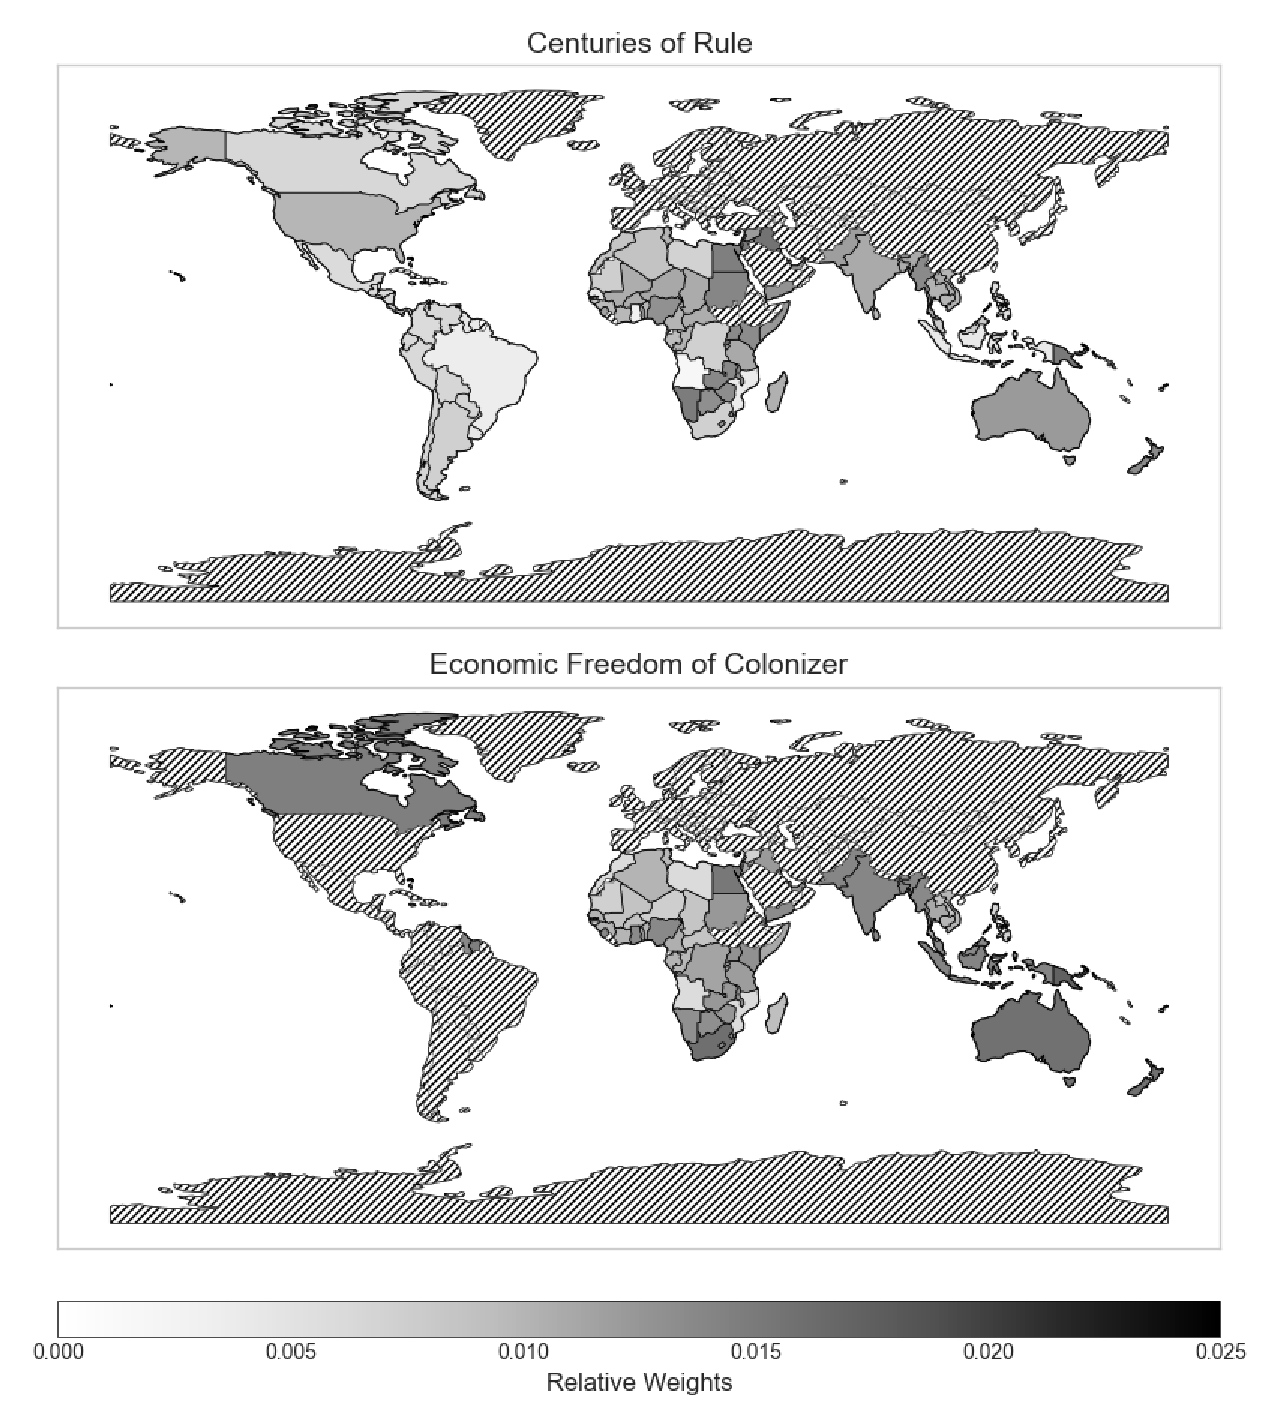
\includegraphics[width=\textwidth]{Plots/output.eps}
    \caption{Effective Sample and Relative Weights}
    \smallskip
    {\footnotesize \textit{Notes:} Stripped countries excluded from effective sample. Top panel refers to Column (1) of Table \ref{tab:Tab3}, bottom panel to Column (2) of Table \ref{tab:Tab4}.}
    \label{fig:FigB1}
\end{figure}

\vspace{5cm}
\begin{sidewaystable}[h!]
\begin{threeparttable}
\begin{center}
\begin{minipage}{\textwidth}
\small
\caption{Economic Freedom of Colonizer and Economic Freedom: Individual Areas and Standard Deviation across Areas, 2000-2019 averages}
\label{tab:TabB1}
\begin{tabular*}{\textwidth}{@{\extracolsep{\fill}}lccccccc@{\extracolsep{\fill}}}
\hline\hline
            &\multicolumn{1}{c}{Area 1}&\multicolumn{1}{c}{Area 2}&\multicolumn{1}{c}{Area 3}&\multicolumn{1}{c}{Area 4}&\multicolumn{1}{c}{Area 5}&\multicolumn{1}{c}{Stand. Dev.}&\multicolumn{1}{c}{EFW}\\
            &\multicolumn{1}{c}{(1)}&\multicolumn{1}{c}{(2)}&\multicolumn{1}{c}{(3)}&\multicolumn{1}{c}{(4)}&\multicolumn{1}{c}{(5)}&\multicolumn{1}{c}{(6)}&\multicolumn{1}{c}{(7)}\\
\hline
HIEL Colonier &       0.325         &       1.124\sym{***}&       0.505\sym{*}  &       0.740\sym{**} &       0.881\sym{***}&      -0.146         &       0.716\sym{***}\\
            &     (0.209)         &     (0.296)         &     (0.259)         &     (0.302)         &     (0.207)         &    (0.0916)         &     (0.193)         \\
[0.25em]
\hline
\(N\)       &          87         &          87         &          87         &          87         &          87         &          87         &          87         \\
\(R^{2}\)   &       0.029         &       0.176         &       0.043         &       0.078         &       0.158         &       0.034         &       0.154         \\
\hline\hline
\end{tabular*}
\begin{tablenotes}
\small
\item \textit{Notes}: Robust standard errors in parenthesis. *, **, and *** indicate statistical significance at the 10, 5, and 1\% levels, respectively. Countries with multiple colonizers are classified as colonies of their \textit{main} colonizer, following \cite{laporta1999quality}. Dependent variables: Columns (1) to (5) is the 2000-2019 average the five individual areas of the \textit{Economic Freedom of the World} (EFW): (1) Size of Government, (2) Legal System and Property Rights, (3) Sound Money, (4) Freedom to Trade Internationally, and (5) Regulation. The scores range from 0 to 10. Column (6) is the 2000-2019 average of the within-year standard deviation among the five areas, following \cite{bolen2020does}. Column (7) is the 2000-2019 average score for all five areas, reproducing Table \ref{tab:Tab3}, Column (1), for convenient comparison between the magnitudes of individual areas and the overall EFW score.
\end{tablenotes}
\end{minipage}
\end{center}
\end{threeparttable}
\end{sidewaystable}

\clearpage
\begin{sidewaystable}[h!]
\begin{threeparttable}
\begin{center}
\begin{minipage}{\textwidth}
\small
\caption{Length of European Colonial Rule and Economic Freedom: Individual Areas and Standard Deviation across Areas, 2000-2019 averages}
\label{tab:TabB2}
\begin{tabular*}{\textwidth}{@{\extracolsep{\fill}}lccccccc@{\extracolsep{\fill}}}
\hline\hline
            &\multicolumn{1}{c}{Area 1}&\multicolumn{1}{c}{Area 2}&\multicolumn{1}{c}{Area 3}&\multicolumn{1}{c}{Area 4}&\multicolumn{1}{c}{Area 5}&\multicolumn{1}{c}{Stand. Dev.}&\multicolumn{1}{c}{EFW}\\
            &\multicolumn{1}{c}{(1)}&\multicolumn{1}{c}{(2)}&\multicolumn{1}{c}{(3)}&\multicolumn{1}{c}{(4)}&\multicolumn{1}{c}{(5)}&\multicolumn{1}{c}{(6)}&\multicolumn{1}{c}{(7)}\\
\hline
Centuries of rule &       0.167\sym{*}  &       0.284\sym{**} &       0.105         &       0.198         &       0.229\sym{**} &     -0.0729\sym{**} &       0.196\sym{**} \\
            &    (0.0998)         &     (0.109)         &     (0.110)         &     (0.122)         &    (0.0892)         &    (0.0337)         &    (0.0790)         \\
[0.125em]
Former British &      -0.434\sym{***}&       2.610\sym{***}&       1.896\sym{***}&       1.268\sym{***}&       2.203\sym{***}&      -0.559\sym{***}&       1.511\sym{***}\\
            &     (0.136)         &     (0.246)         &     (0.242)         &     (0.253)         &     (0.200)         &    (0.0692)         &     (0.165)         \\
[0.125em]
Former French &      -0.575\sym{***}&       1.431\sym{***}&       1.202\sym{***}&       0.588\sym{***}&       1.368\sym{***}&      -0.519\sym{***}&       0.805\sym{***}\\
            &     (0.209)         &     (0.161)         &     (0.180)         &     (0.184)         &     (0.174)         &    (0.0836)         &     (0.133)         \\
[0.125em]
Former German &      -0.907\sym{***}&       1.999\sym{***}&       1.784\sym{***}&       0.163         &       1.965\sym{***}&      -0.533\sym{***}&       0.997\sym{***}\\
            &     (0.315)         &     (0.600)         &     (0.262)         &     (0.342)         &     (0.285)         &     (0.155)         &     (0.265)         \\
[0.125em]
Former Italian &      -2.004\sym{***}&       1.149\sym{***}&       0.981\sym{***}&      -2.930\sym{***}&       1.098\sym{***}&      -0.112\sym{***}&      -0.382\sym{***}\\
            &    (0.0389)         &    (0.0424)         &    (0.0429)         &    (0.0476)         &    (0.0348)         &    (0.0131)         &    (0.0308)         \\
[0.125em]
Former Dutch &      -0.865         &       1.569\sym{***}&       2.092\sym{***}&       0.826         &       1.172\sym{***}&      -0.268         &       0.967\sym{***}\\
            &     (1.058)         &     (0.352)         &     (0.278)         &     (0.557)         &     (0.327)         &     (0.162)         &     (0.292)         \\
[0.125em]
Former Portuguese &      -1.333\sym{***}&       1.259\sym{**} &       1.175\sym{**} &       0.650         &       0.380         &      -0.359\sym{*}  &       0.437         \\
            &     (0.434)         &     (0.518)         &     (0.550)         &     (0.533)         &     (0.342)         &     (0.192)         &     (0.305)         \\
[0.125em]
Former Spanish &      0.0172         &       1.837\sym{***}&       2.264\sym{***}&       1.654\sym{***}&       1.316\sym{***}&      -0.294\sym{**} &       1.424\sym{***}\\
            &     (0.331)         &     (0.331)         &     (0.457)         &     (0.388)         &     (0.282)         &     (0.118)         &     (0.292)         \\
[0.125em]
\hline
\(N\)       &         107         &         107         &         107         &         107         &         107         &         107         &         107         \\
\(R^{2}\)   &       0.280         &       0.176         &       0.246         &       0.119         &       0.235         &       0.247         &       0.079         \\
\hline\hline
\end{tabular*}
\begin{tablenotes}
\small
\item \textit{Notes}: Robust standard errors in parenthesis. *, **, and *** indicate statistical significance at the 10, 5, and 1\% levels, respectively. Baseline is former Belgian colonies.Countries with multiple colonizers are classified as colonies of their \textit{main} colonizer, following \cite{laporta1999quality}. Dependent variables: Columns (1) to (5) is the 2000-2019 average the five individual areas of the \textit{Economic Freedom of the World} (EFW): (1) Size of Government, (2) Legal System and Property Rights, (3) Sound Money, (4) Freedom to Trade Internationally, and (5) Regulation. The scores range from 0 to 10. Column (6) is the 2000-2019 average of the within-year standard deviation among the five areas, following \cite{bolen2020does}. Column (7) is the 2000-2019 average score for all five areas, reproducing Table \ref{tab:Tab4}, Column (2), but including the values for the colonizer dummies.
\end{tablenotes}
\end{minipage}
\end{center}
\end{threeparttable}
\end{sidewaystable}

\clearpage
{
\def\sym#1{\ifmmode^{#1}\else\(^{#1}\)\fi}
\begin{tabular}{l*{7}{c}}
\hline\hline
            &\multicolumn{1}{c}{(1)}&\multicolumn{1}{c}{(2)}&\multicolumn{1}{c}{(3)}&\multicolumn{1}{c}{(4)}&\multicolumn{1}{c}{(5)}&\multicolumn{1}{c}{(6)}&\multicolumn{1}{c}{(7)}\\
            &\multicolumn{1}{c}{Area1}&\multicolumn{1}{c}{Area2}&\multicolumn{1}{c}{Area3}&\multicolumn{1}{c}{Area4}&\multicolumn{1}{c}{Area5}&\multicolumn{1}{c}{std}&\multicolumn{1}{c}{avg\_efw}\\
\hline
centuries   &       0.167\sym{*}  &       0.284\sym{**} &       0.105         &       0.198         &       0.229\sym{**} &     -0.0729\sym{**} &       0.196\sym{**} \\
            &    (0.0998)         &     (0.109)         &     (0.110)         &     (0.122)         &    (0.0892)         &    (0.0337)         &    (0.0790)         \\
[1em]
1.colonizer &           0         &           0         &           0         &           0         &           0         &           0         &           0         \\
            &         (.)         &         (.)         &         (.)         &         (.)         &         (.)         &         (.)         &         (.)         \\
[1em]
2.colonizer &      -0.434\sym{***}&       2.610\sym{***}&       1.896\sym{***}&       1.268\sym{***}&       2.203\sym{***}&      -0.559\sym{***}&       1.511\sym{***}\\
            &     (0.136)         &     (0.246)         &     (0.242)         &     (0.253)         &     (0.200)         &    (0.0692)         &     (0.165)         \\
[1em]
3.colonizer &      -0.575\sym{***}&       1.431\sym{***}&       1.202\sym{***}&       0.588\sym{***}&       1.368\sym{***}&      -0.519\sym{***}&       0.805\sym{***}\\
            &     (0.209)         &     (0.161)         &     (0.180)         &     (0.184)         &     (0.174)         &    (0.0836)         &     (0.133)         \\
[1em]
4.colonizer &      -0.907\sym{***}&       1.999\sym{***}&       1.784\sym{***}&       0.163         &       1.965\sym{***}&      -0.533\sym{***}&       0.997\sym{***}\\
            &     (0.315)         &     (0.600)         &     (0.262)         &     (0.342)         &     (0.285)         &     (0.155)         &     (0.265)         \\
[1em]
5.colonizer &      -2.004\sym{***}&       1.149\sym{***}&       0.981\sym{***}&      -2.930\sym{***}&       1.098\sym{***}&      -0.112\sym{***}&      -0.382\sym{***}\\
            &    (0.0389)         &    (0.0424)         &    (0.0429)         &    (0.0476)         &    (0.0348)         &    (0.0131)         &    (0.0308)         \\
[1em]
6.colonizer &      -0.865         &       1.569\sym{***}&       2.092\sym{***}&       0.826         &       1.172\sym{***}&      -0.268         &       0.967\sym{***}\\
            &     (1.058)         &     (0.352)         &     (0.278)         &     (0.557)         &     (0.327)         &     (0.162)         &     (0.292)         \\
[1em]
7.colonizer &      -1.333\sym{***}&       1.259\sym{**} &       1.175\sym{**} &       0.650         &       0.380         &      -0.359\sym{*}  &       0.437         \\
            &     (0.434)         &     (0.518)         &     (0.550)         &     (0.533)         &     (0.342)         &     (0.192)         &     (0.305)         \\
[1em]
8.colonizer &      0.0172         &       1.837\sym{***}&       2.264\sym{***}&       1.654\sym{***}&       1.316\sym{***}&      -0.294\sym{**} &       1.424\sym{***}\\
            &     (0.331)         &     (0.331)         &     (0.457)         &     (0.388)         &     (0.282)         &     (0.118)         &     (0.292)         \\
[1em]
\_cons      &       7.092\sym{***}&       2.046\sym{***}&       5.757\sym{***}&       5.164\sym{***}&       4.534\sym{***}&       2.047\sym{***}&       4.916\sym{***}\\
            &    (0.0748)         &    (0.0815)         &    (0.0824)         &    (0.0916)         &    (0.0669)         &    (0.0252)         &    (0.0593)         \\
\hline
\(N\)       &         107         &         107         &         107         &         107         &         107         &         107         &         107         \\
\(R^{2}\)   &       0.174         &       0.240         &       0.136         &       0.258         &       0.248         &       0.080         &       0.264         \\
\hline\hline
\multicolumn{8}{l}{\footnotesize Standard errors in parentheses}\\
\multicolumn{8}{l}{\footnotesize \sym{*} \(p<0.10\), \sym{**} \(p<0.05\), \sym{***} \(p<0.01\)}\\
\end{tabular}
}


\clearpage
{
\def\sym#1{\ifmmode^{#1}\else\(^{#1}\)\fi}
\begin{tabular}{l*{4}{c}}
\hline\hline
            &\multicolumn{1}{c}{(1)}&\multicolumn{1}{c}{(2)}&\multicolumn{1}{c}{(3)}&\multicolumn{1}{c}{(4)}\\
            &\multicolumn{1}{c}{avg\_efw}&\multicolumn{1}{c}{avg\_efw}&\multicolumn{1}{c}{avg\_efw}&\multicolumn{1}{c}{avg\_efw}\\
\hline
efw\_colonizer&       0.716\sym{***}&       0.521\sym{*}  &       1.145\sym{**} &       0.725         \\
            &     (0.181)         &     (0.251)         &     (0.419)         &     (0.510)         \\
[1em]
america     &                     &      0.0338         &      -0.339         &      -0.568         \\
            &                     &     (0.220)         &     (0.804)         &     (1.035)         \\
[1em]
africa      &                     &      -0.327         &      -0.604         &      -0.601         \\
            &                     &     (0.218)         &     (0.480)         &     (1.027)         \\
[1em]
asia        &                     &      -0.137         &      -0.743         &      -0.794         \\
            &                     &     (0.215)         &     (0.737)         &     (1.116)         \\
[1em]
lat\_abst    &                     &       1.082         &      -3.959\sym{**} &      -2.623         \\
            &                     &     (1.247)         &     (1.354)         &     (2.233)         \\
[1em]
landlock    &                     &       0.339         &       0.915\sym{***}&       1.002\sym{*}  \\
            &                     &     (0.340)         &     (0.217)         &     (0.490)         \\
[1em]
island      &                     &       0.959\sym{**} &       1.333\sym{***}&       1.292\sym{**} \\
            &                     &     (0.319)         &     (0.310)         &     (0.333)         \\
[1em]
ruggedness  &                     &                     &    -0.00247         &    -0.00194         \\
            &                     &                     &   (0.00154)         &   (0.00154)         \\
[1em]
logem4      &                     &                     &     -0.0930         &      -0.132         \\
            &                     &                     &     (0.233)         &     (0.147)         \\
[1em]
lpd1500s    &                     &                     &      -0.164         &      -0.127         \\
            &                     &                     &     (0.230)         &     (0.226)         \\
[1em]
humid1      &                     &                     &     -0.0121         &     0.00552         \\
            &                     &                     &    (0.0121)         &    (0.0332)         \\
[1em]
humid2      &                     &                     &      0.0653\sym{***}&      0.0528         \\
            &                     &                     &    (0.0100)         &    (0.0289)         \\
[1em]
humid3      &                     &                     &      0.0444\sym{*}  &      0.0382         \\
            &                     &                     &    (0.0177)         &    (0.0214)         \\
[1em]
humid4      &                     &                     &     -0.0214         &    -0.00879         \\
            &                     &                     &    (0.0216)         &    (0.0143)         \\
[1em]
temp1       &                     &                     &      -0.278         &      -0.304         \\
            &                     &                     &     (0.206)         &     (0.235)         \\
[1em]
temp2       &                     &                     &      -0.101\sym{**} &     -0.0562         \\
            &                     &                     &    (0.0276)         &    (0.0841)         \\
[1em]
temp3       &                     &                     &       0.263\sym{**} &       0.275\sym{**} \\
            &                     &                     &    (0.0850)         &    (0.0848)         \\
[1em]
temp4       &                     &                     &      0.0335         &      0.0407         \\
            &                     &                     &    (0.0422)         &    (0.0565)         \\
[1em]
temp5       &                     &                     &      0.0798         &      0.0907         \\
            &                     &                     &    (0.0482)         &    (0.0619)         \\
[1em]
steplow     &                     &                     &      0.0457         &      0.0144         \\
            &                     &                     &     (0.162)         &     (0.261)         \\
[1em]
deslow      &                     &                     &      0.0164         &       0.331         \\
            &                     &                     &     (0.276)         &     (0.284)         \\
[1em]
stepmid     &                     &                     &       1.324         &       1.190         \\
            &                     &                     &     (1.800)         &     (2.805)         \\
[1em]
desmid      &                     &                     &           0         &           0         \\
            &                     &                     &         (.)         &         (.)         \\
[1em]
drystep     &                     &                     &      -0.112         &      -0.295         \\
            &                     &                     &     (0.220)         &     (0.342)         \\
[1em]
hiland      &                     &                     &           0         &           0         \\
            &                     &                     &         (.)         &         (.)         \\
[1em]
drywint     &                     &                     &       26.28         &       28.64         \\
            &                     &                     &     (25.17)         &     (42.51)         \\
[1em]
goldm       &                     &                     &      -0.539         &      -0.603         \\
            &                     &                     &     (0.536)         &     (0.918)         \\
[1em]
iron        &                     &                     &      -0.110\sym{**} &     -0.0701         \\
            &                     &                     &    (0.0375)         &     (0.134)         \\
[1em]
silv        &                     &                     &           0         &           0         \\
            &                     &                     &         (.)         &         (.)         \\
[1em]
zinc        &                     &                     &           0         &           0         \\
            &                     &                     &         (.)         &         (.)         \\
[1em]
oilres      &                     &                     & -0.00000157\sym{**} & -0.00000120\sym{*}  \\
            &                     &                     &(0.000000524)         &(0.000000559)         \\
[1em]
1.long\_colonizer&                     &                     &           0         &           0         \\
            &                     &                     &         (.)         &         (.)         \\
[1em]
2.long\_colonizer&                     &                     &      -1.280         &      -1.975         \\
            &                     &                     &     (0.823)         &     (1.346)         \\
[1em]
3.long\_colonizer&                     &                     &      -1.637\sym{*}  &      -2.143         \\
            &                     &                     &     (0.806)         &     (1.212)         \\
[1em]
6.long\_colonizer&                     &                     &      -2.466\sym{*}  &      -2.684         \\
            &                     &                     &     (1.148)         &     (1.384)         \\
[1em]
7.long\_colonizer&                     &                     &      -1.213         &      -2.244         \\
            &                     &                     &     (0.687)         &     (1.468)         \\
[1em]
8.long\_colonizer&                     &                     &      -1.166         &      -2.183         \\
            &                     &                     &     (0.811)         &     (1.424)         \\
[1em]
legor\_fr    &                     &                     &                     &       0.203         \\
            &                     &                     &                     &     (0.911)         \\
[1em]
legor\_uk    &                     &                     &                     &       0.958         \\
            &                     &                     &                     &     (0.849)         \\
[1em]
\_cons      &       0.984         &       2.129         &      -6.683         &      -5.792         \\
            &     (1.408)         &     (2.093)         &     (6.454)         &     (5.374)         \\
\hline
\(N\)       &          87         &          70         &          53         &          53         \\
\(R^{2}\)   &       0.154         &       0.435         &       0.830         &       0.848         \\
\hline\hline
\multicolumn{5}{l}{\footnotesize Standard errors in parentheses}\\
\multicolumn{5}{l}{\footnotesize \sym{*} \(p<0.10\), \sym{**} \(p<0.05\), \sym{***} \(p<0.01\)}\\
\end{tabular}
}


\clearpage
{
\def\sym#1{\ifmmode^{#1}\else\(^{#1}\)\fi}
\begin{tabular}{l*{8}{c}}
\hline\hline
            &\multicolumn{1}{c}{(1)}&\multicolumn{1}{c}{(2)}&\multicolumn{1}{c}{(3)}&\multicolumn{1}{c}{(4)}&\multicolumn{1}{c}{(5)}&\multicolumn{1}{c}{(6)}&\multicolumn{1}{c}{(7)}&\multicolumn{1}{c}{(8)}\\
            &\multicolumn{1}{c}{first}&\multicolumn{1}{c}{first}&\multicolumn{1}{c}{first}&\multicolumn{1}{c}{first}&\multicolumn{1}{c}{centuries}&\multicolumn{1}{c}{centuries}&\multicolumn{1}{c}{centuries}&\multicolumn{1}{c}{centuries}\\
\hline
lat\_abst    &       95.37         &                     &                     &                     &      -0.579         &                     &                     &                     \\
            &     (68.24)         &                     &                     &                     &     (0.605)         &                     &                     &                     \\
[1em]
landlock    &       61.08\sym{***}&                     &                     &                     &      -0.629\sym{***}&                     &                     &                     \\
            &     (18.73)         &                     &                     &                     &     (0.155)         &                     &                     &                     \\
[1em]
island      &      -23.97         &                     &                     &                     &       0.521         &                     &                     &                     \\
            &     (43.38)         &                     &                     &                     &     (0.414)         &                     &                     &                     \\
[1em]
america     &      -289.1\sym{***}&                     &                     &                     &       2.544\sym{***}&                     &                     &                     \\
            &     (47.96)         &                     &                     &                     &     (0.418)         &                     &                     &                     \\
[1em]
africa      &      -16.93         &                     &                     &                     &       0.866\sym{*}  &                     &                     &                     \\
            &     (55.40)         &                     &                     &                     &     (0.488)         &                     &                     &                     \\
[1em]
asia        &      -82.22         &                     &                     &                     &       0.994\sym{**} &                     &                     &                     \\
            &     (51.53)         &                     &                     &                     &     (0.418)         &                     &                     &                     \\
[1em]
humid1      &                     &      -3.673         &                     &                     &                     &      0.0214         &                     &                     \\
            &                     &     (3.203)         &                     &                     &                     &    (0.0278)         &                     &                     \\
[1em]
humid2      &                     &      -0.168         &                     &                     &                     &      0.0142         &                     &                     \\
            &                     &     (5.002)         &                     &                     &                     &    (0.0462)         &                     &                     \\
[1em]
humid3      &                     &      -0.826         &                     &                     &                     &      0.0150         &                     &                     \\
            &                     &     (3.547)         &                     &                     &                     &    (0.0310)         &                     &                     \\
[1em]
humid4      &                     &       3.030         &                     &                     &                     &     -0.0208         &                     &                     \\
            &                     &     (3.662)         &                     &                     &                     &    (0.0318)         &                     &                     \\
[1em]
temp1       &                     &       9.101         &                     &                     &                     &      0.0588         &                     &                     \\
            &                     &     (19.72)         &                     &                     &                     &     (0.174)         &                     &                     \\
[1em]
temp2       &                     &      -8.849         &                     &                     &                     &      0.0398         &                     &                     \\
            &                     &     (6.411)         &                     &                     &                     &    (0.0450)         &                     &                     \\
[1em]
temp3       &                     &       6.678         &                     &                     &                     &     -0.0787         &                     &                     \\
            &                     &     (9.225)         &                     &                     &                     &    (0.0874)         &                     &                     \\
[1em]
temp4       &                     &       3.083         &                     &                     &                     &     -0.0711         &                     &                     \\
            &                     &     (7.516)         &                     &                     &                     &    (0.0754)         &                     &                     \\
[1em]
temp5       &                     &      -5.678         &                     &                     &                     &      0.0450         &                     &                     \\
            &                     &     (5.282)         &                     &                     &                     &    (0.0441)         &                     &                     \\
[1em]
steplow     &                     &       31.56         &                     &                     &                     &      -0.184         &                     &                     \\
            &                     &     (38.63)         &                     &                     &                     &     (0.309)         &                     &                     \\
[1em]
deslow      &                     &      -54.07         &                     &                     &                     &       0.381         &                     &                     \\
            &                     &     (44.36)         &                     &                     &                     &     (0.347)         &                     &                     \\
[1em]
stepmid     &                     &      -75.52         &                     &                     &                     &       0.620         &                     &                     \\
            &                     &     (64.40)         &                     &                     &                     &     (0.458)         &                     &                     \\
[1em]
desmid      &                     &      -195.1\sym{***}&                     &                     &                     &       0.808\sym{*}  &                     &                     \\
            &                     &     (54.37)         &                     &                     &                     &     (0.414)         &                     &                     \\
[1em]
drystep     &                     &       85.52\sym{**} &                     &                     &                     &      -0.600         &                     &                     \\
            &                     &     (41.81)         &                     &                     &                     &     (0.424)         &                     &                     \\
[1em]
hiland      &                     &           0         &                     &                     &                     &           0         &                     &                     \\
            &                     &         (.)         &                     &                     &                     &         (.)         &                     &                     \\
[1em]
drywint     &                     &      -96.37         &                     &                     &                     &       0.881\sym{*}  &                     &                     \\
            &                     &     (65.38)         &                     &                     &                     &     (0.528)         &                     &                     \\
[1em]
goldm       &                     &                     &      -3.166\sym{***}&                     &                     &                     &      0.0230\sym{***}&                     \\
            &                     &                     &     (0.441)         &                     &                     &                     &   (0.00448)         &                     \\
[1em]
iron        &                     &                     &       10.93\sym{*}  &                     &                     &                     &     -0.0784         &                     \\
            &                     &                     &     (5.844)         &                     &                     &                     &    (0.0497)         &                     \\
[1em]
silv        &                     &                     &      -18.71\sym{***}&                     &                     &                     &       0.101\sym{***}&                     \\
            &                     &                     &     (3.195)         &                     &                     &                     &    (0.0218)         &                     \\
[1em]
zinc        &                     &                     &       1.993         &                     &                     &                     &     -0.0195         &                     \\
            &                     &                     &     (5.791)         &                     &                     &                     &    (0.0622)         &                     \\
[1em]
oilres      &                     &                     &  0.00000262         &                     &                     &                     &-0.000000109         &                     \\
            &                     &                     & (0.0000348)         &                     &                     &                     &(0.000000223)         &                     \\
[1em]
lpd1500s    &                     &                     &                     &       31.00\sym{***}&                     &                     &                     &      -0.208\sym{***}\\
            &                     &                     &                     &     (8.410)         &                     &                     &                     &    (0.0721)         \\
[1em]
\_cons      &      1830.3\sym{***}&      1703.7\sym{***}&      1748.4\sym{***}&      1722.9\sym{***}&       0.573         &      0.0612         &       1.831\sym{***}&       1.964\sym{***}\\
            &     (58.75)         &     (263.4)         &     (18.40)         &     (18.04)         &     (0.506)         &     (2.288)         &     (0.149)         &     (0.146)         \\
\hline
\(N\)       &          90         &          89         &          89         &          86         &          90         &          89         &          89         &          86         \\
\(R^{2}\)   &       0.661         &       0.319         &       0.061         &       0.090         &       0.509         &       0.256         &       0.030         &       0.064         \\
\hline\hline
\multicolumn{9}{l}{\footnotesize Standard errors in parentheses}\\
\multicolumn{9}{l}{\footnotesize \sym{*} \(p<0.10\), \sym{**} \(p<0.05\), \sym{***} \(p<0.01\)}\\
\end{tabular}
}


\clearpage
{
\def\sym#1{\ifmmode^{#1}\else\(^{#1}\)\fi}
\begin{tabular}{l*{3}{c}}
\hline\hline
            &\multicolumn{1}{c}{(1)}&\multicolumn{1}{c}{(2)}&\multicolumn{1}{c}{(3)}\\
            &\multicolumn{1}{c}{std}&\multicolumn{1}{c}{std}&\multicolumn{1}{c}{std}\\
\hline
multiple    &      -0.141         &      -0.169\sym{*}  &     -0.0813         \\
            &    (0.0868)         &    (0.0990)         &     (0.166)         \\
[1em]
1.colonizer &                     &           0         &           0         \\
            &                     &         (.)         &         (.)         \\
[1em]
2.colonizer &                     &      -0.566\sym{***}&      -0.551\sym{***}\\
            &                     &    (0.0697)         &    (0.0693)         \\
[1em]
3.colonizer &                     &      -0.514\sym{***}&      -0.512\sym{***}\\
            &                     &    (0.0838)         &    (0.0854)         \\
[1em]
4.colonizer &                     &      -0.367\sym{**} &      -0.452\sym{**} \\
            &                     &     (0.182)         &     (0.226)         \\
[1em]
5.colonizer &                     &      0.0857         &     -0.0234         \\
            &                     &    (0.0990)         &     (0.186)         \\
[1em]
6.colonizer &                     &      -0.451\sym{***}&      -0.314         \\
            &                     &     (0.136)         &     (0.203)         \\
[1em]
7.colonizer &                     &      -0.536\sym{***}&      -0.403\sym{*}  \\
            &                     &     (0.197)         &     (0.222)         \\
[1em]
8.colonizer &                     &      -0.446\sym{***}&      -0.330\sym{**} \\
            &                     &    (0.0886)         &     (0.152)         \\
[1em]
centuries   &                     &                     &     -0.0546         \\
            &                     &                     &    (0.0588)         \\
[1em]
\_cons      &       1.475\sym{***}&       1.993         &       2.034\sym{***}\\
            &    (0.0456)         &         (.)         &    (0.0441)         \\
\hline
\(N\)       &         107         &         107         &         107         \\
\(R^{2}\)   &       0.020         &       0.072         &       0.083         \\
\hline\hline
\multicolumn{4}{l}{\footnotesize Standard errors in parentheses}\\
\multicolumn{4}{l}{\footnotesize \sym{*} \(p<0.10\), \sym{**} \(p<0.05\), \sym{***} \(p<0.01\)}\\
\end{tabular}
}


\clearpage
\subsection{Determinants of Colonial Rule}

\justifying 
\doublespacing
Here, I explore which variables are able to explain the length and timing of colonial tenure. Table \ref{tab:TabB7} reports the results. Panel A shows the determinants of the timing of colonization (year first colonized) and Panel B the length of colonial rule. I consider four sets of determinants for each: location, climate/soil, natural resources, and pre-colonial development. Location includes absolute latitude, dummies for island and landlocked colonies, and continent dummies (not reported). The major finding is that landlocked countries were colonized later and for shorter periods of time. The second column of each panel includes four indicators of humidity, five indicators of temperature, and six indicators of climate/soil. I report $p$-values for whether each of these three groups are significant jointly significant. Humidity matters for both the timing and length of colonial rule, and climate/soil for timing. Natural resources are considered in the third column of each panel. The results point out that colonies with gold and silver were colonized first.\footnote{However, when including a dummy for America silver ceases to be significant.} 

Finally, I consider the role of greater pre-colonial development using a the (log) population density in the 1500's. As \citet[p. 1232]{acemoglu2002reversal} argues ``only areas with high agricultural productivity and a developed transportation network can support large urban populations.'' I find that colonies with greater population density in the pre-colonial era were colonized later and held for shorter periods of time. Fully specificied models account for 71\% of the variation of timing of colonization, and 59\% of the length of colonization. 

\clearpage
\begin{sidewaystable}[h!]
\begin{threeparttable}
\begin{center}
\begin{minipage}{\textwidth}
\small
\caption{Determinants of Timing and Length of Colonization}
\label{tab:TabB7}
\begin{tabular*}{\textwidth}{@{\extracolsep{\fill}}lcccccccccccc@{\extracolsep{\fill}}}
\hline\hline
\textit{Dep. Variable:}    &\multicolumn{4}{c}{\textit{Panel A: Year First Colonized}}
            &\multicolumn{4}{c}{\textit{Panel B: Length of Colonial Rule}}\\
            \cmidrule{2-5} \cmidrule{6-9}
            &\multicolumn{1}{c}{Location}
            &\multicolumn{1}{c}{Climate}
            &\multicolumn{1}{c}{Natural}
            &\multicolumn{1}{c}{Pre-Colonial}
            &\multicolumn{1}{c}{Location}
            &\multicolumn{1}{c}{Climate}
            &\multicolumn{1}{c}{Natural}
            &\multicolumn{1}{c}{Pre-Colonial}\\
            & & and Soil & Resources& Development && and Soil&Resources& Development \\
    
\hline

Abs. Latitude   &       95.37         &                     &                     &                     &      -0.579         &                     &                     &                     \\
            &     (68.24)         &                     &                     &                     &     (0.605)         &                     &                     &                     \\
[0.5em]
Landlocked    &       61.08\sym{***}&                     &                     &                     &      -0.629\sym{***}&                     &                     &                     \\
            &     (18.73)         &                     &                     &                     &     (0.155)         &                     &                     &                     \\
[0.5em]
Island      &      -23.97         &                     &                     &                     &       0.521         &                     &                     &                     \\
            &     (43.38)         &                     &                     &                     &     (0.414)         &                     &                     &                     \\
[0.5em]
%America     &      -289.1\sym{***}&                     &                     &                     &       2.544\sym{***}&                     &                     &                     \\
%            &     (47.96)         &                     &                     &                     &     (0.418)         &                     &                     &                     \\
%[0.5em]
%Africa      &      -16.93         &                     &                     &                     &       0.866\sym{*}  &                     &                     &                     \\
%            &     (55.40)         &                     &                     &                     &     (0.488)         &                     &                     &                     \\
%[0.5em]
%Asia        &      -82.22         &                     &                     &                     &       0.994\sym{**} &                     &                     &                     \\
%            &     (51.53)         &                     &                     &                     &     (0.418)         &                     &                     &                     \\
%[0.5em]
$P$-val. humidity &&(0.002)***&&&& (0.002)*** & \\
$P$-val. temperature &&(0.311)\;\;\;\;\; &&&& (0.572)\;\;\;\;\; & \\
$P$-val. climate/soil &&(0.000)***&&&& (0.313)\;\;\;\;\; & \\
[0.5em]
Gold       &                     &                     &      -3.166\sym{***}&                     &                     &                     &      0.023\sym{***}&                     \\
            &                     &                     &     (0.441)         &                     &                     &                     &   (0.004)         &                     \\
[0.5em]
Iron        &                     &                     &       10.93\sym{*}  &                     &                     &                     &     -0.078         &                     \\
            &                     &                     &     (5.844)         &                     &                     &                     &    (0.0497)         &                     \\
[0.5em]
Silver        &                     &                     &      -18.71\sym{***}&                     &                     &                     &       0.101\sym{***}&                     \\
            &                     &                     &     (3.195)         &                     &                     &                     &    (0.022)         &                     \\
[0.5em]
Zinc        &                     &                     &       1.993         &                     &                     &                     &     -0.020         &                     \\
            &                     &                     &     (5.791)         &                     &                     &                     &    (0.0622)         &                     \\
[0.5em]
Oil      &                     &                     &  0.000   &                     &                     &                     &0.000        &                     \\
            &                     &                     & (0.000)         &                     &                     &                     &(0.000)         &                     \\
[0.5em]
Pop. Density (1500s)    &                     &                     &                     &       31.00\sym{***}&                     &                     &                     &      -0.208\sym{***}\\
            &                     &                     &                     &     (8.410)         &                     &                     &                     &    (0.0721)         \\
\hline
\(N\)       &          90         &          89         &          89         &          86         &          90         &          89         &          89         &          86         \\
\(R^{2}\)   &       0.661         &       0.319         &       0.061         &       0.090         &       0.509         &       0.256         &       0.030         &       0.064         \\

\hline
\end{tabular*}
\begin{tablenotes}
\small
\item \textit{Notes}: Robust standard errors in parenthesis. *, **, and *** indicate statistical significance at the 10, 5, and 1\% levels, respectively. \textit{Location:} includes dummies for America, Asia, and Africa (not reported). \textit{Climate and soil}: four indicators of humidity, five indicators of temperature, and six indicators of climate/soil. Reports $p$-values for the joint significance of each set of indicators. Population density in the 1500's from \cite{acemoglu2002reversal}.
\end{tablenotes}
\end{minipage}
\end{center}
\end{threeparttable}
\end{sidewaystable}

% ================================================================
% --- THE END
\end{document}